%%This is a very basic article template.
%%There is just one section and two subsections.
\documentclass[parskip=full]{scrartcl}
\usepackage[table]{xcolor}

\usepackage{amsmath}
\usepackage{amsfonts}
\usepackage{studarbeit}
\usepackage{graphicx}
\usepackage{wrapfig}
\usepackage{lscape}
\usepackage{rotating}
\usepackage{epstopdf}
\usepackage[binary-units=true]{siunitx}
 \usepackage[autostyle=true,german=quotes]{csquotes}
 \usepackage{longtable, booktabs}
\usepackage[most]{tcolorbox}
\definecolor{testgrauRGB}{rgb}{0.9,0.9,0.9}
\definecolor{testgrauCMYK}{cmyk}{0.0,0.0,0.0,0.30}
% \newcommand{\grayColBox}{1}{ \begin{tcolorbox}[enhanced jigsaw, %
% % needed
%    % to really the frame off!
%  colback=testgrauRGB % black background
%  coltext=black, % white text
%  %halign=center, % center
% % fontupper={\Huge \bfseries}, % change the font here
%  sharp corners, % no rounded corners
%  colframe=black, % not really necessary
%  boxrule=0pt % frame off 
%  ]\texttt{#1}
%  \end{tcolorbox}
% }
%% zwei verschiedene Grautoene in zwei Farbsystemen:






% ---------------------------------------------------------------------------
% TexDoc macros start - everything below this point should be copied to your
% own document and adapted to your style/language if needed
% ---------------------------------------------------------------------------

% Environment used to simulate html <p> </p>
\newenvironment{texdocp}{}{

}
% Environment for packages
\newenvironment{texdocpackage}[1]{%
	\gdef\packagename{#1}\subsection{Packet \texttt{#1}}
	\rule{\hsize}{.7mm}
}{}

% Environment for classes, interfaces
% Argument 1: "class" or "interface"
% Argument 2: the name of the class/interface
\newenvironment{texdocclass}[2]{%
	\gdef\classname{#2}
	\subsubsection{\texttt{#1 \textbf{#2}}}
}{\newpage{}}

% Environment for class description
\newenvironment{texdocclassintro}{
	\paragraph*{Beschreibung}
}{
}

% Environment around class fields
\newenvironment{texdocclassfields}{%
	\paragraph*{Attribute}
	\begin{itemize}
}{%
	\end{itemize}
}

% Environment around class methods
\newenvironment{texdocclassmethods}{%
	\paragraph*{Methoden}
	\begin{itemize}[itemsep=10pt]
}{%
	\end{itemize}
}

% Environment around class Constructors
\newenvironment{texdocclassconstructors}{%
	\paragraph*{Konstruktoren}
	\begin{itemize}
}{%
	\end{itemize}
}

% Environment around enum constants
\newenvironment{texdocenums}{%
	\paragraph*{Enum Konstanten}
	\begin{itemize}
}{%
	\end{itemize}
}

% Environment around "See also"-Blocks (\texdocsee invocations)
%  Argument 1: Text preceding the references
\newenvironment{texdocsees}[1]{
	
	\textbf{#1:}
	\begin{itemize}
}{%
	\end{itemize}
}
% Formats a single field
%  Argument 1: modifiers
%  Argument 2: type
%  Argument 3: name
%  Argument 4: Documentation text
\newcommand{\texdocfield}[4]{\item \texttt{#1 #2 \textbf{#3}} \\ #4}

% Formats an enum element
%  Argument 1: name
%  Argument 2: documentation text
\newcommand{\texdocenum}[2]{\item \texttt{\textbf{#1}} \\ #2}

% Formats a single method
%  Argument 1: modifiers
%  Argument 2: return type
%  Argument 3: name
%  Argument 4: part after name (parameters)
%  Argument 5: Documentation text
%  Argument 6: Documentation of parameters/exceptions/return values
\newcommand{\texdocmethod}[6]{\item \texttt{#1 #2 \textbf{#3}#4} \\ #5#6}

% Formats a single constructor
%  Argument 1: modifiers
%  Argument 2: name
%  Argument 3: part after name (parameters)
%  Argument 4: Documentation text
%  Argument 5: Documentation of parameters/exceptions/return values
\newcommand{\texdocconstructor}[5]{\item \texttt{#1 \textbf{#2}#3} \\ #4#5}

% Inserted when @inheritdoc is used
%  Argument 1: Class where the documentation was inherited from
%  Argument 2: Documentation
\newcommand{\texdocinheritdoc}[2]{#2 (\textit{Dokumentation geerbt von \texttt{#1})}}

% Formats a single see-BlockTag
%  Argument 1: text
%  Argument 2: reference label
\newcommand{\texdocsee}[2]{\item \texttt{#1 (\ref{#2})}}

% Environment around \texdocparameter invocations
\newenvironment{texdocparameters}{%
	%\minisec{Parameter}
	\paraRetText{Parameter}
	\begin{tabular}{ll}
}{%
	\end{tabular}
}

% Environment around \texdocthrow invocations
\newenvironment{texdocthrows}{%
        \minisec{Wirft}
        \begin{tabular}{ll}
}{%
        \end{tabular}
}

\newcommand{\texdocreturn}[1]{\paraRetText{Rückgabe} #1}

% Formats a parameter (this gets put inside the input of a \texdocmethod or 
% \texdocconstructor macro)
%  Argument 1: name
%  Argument 2: description text
\newcommand{\texdocparameter}[2]{\texttt{\textbf{#1}} & \begin{minipage}[t]{0.8\textwidth}#2\end{minipage} \\}

% Formats a throws tag
%  Argument 1: exception name
%  Argument 2: description text
\newcommand{\texdocthrow}[2]{\texttt{\textbf{#1}} & \begin{minipage}[t]{0.6\textwidth}#2\end{minipage} \\}

% Used to simulate html <br/>
\newcommand{\texdocbr}{\mbox{}\newline{}}

% Used to simulate html <h[1-9]> - </h[1-9]>
% Argument 1: number of heading (5 for a <h5>)
% Argument 2: heading text
\newcommand{\headref}[2]{\minisec{#2}}

\newcommand{\refdefined}[1]{
\expandafter\ifx\csname r@#1\endcsname\relax
\relax\else
{$($ in \ref{#1}, page \pageref{#1}$)$}
\fi}

\newcommand{\paraRetText}[1]{\\\textbf{#1}:\\}
\setlist[itemize]{leftmargin =*, noitemsep}
\setlength{\parskip}{0.8em}
% ---------------------------------------------------------------------------
% TexDoc macros end
% ---------------------------------------------------------------------------


\begin{document}

\title{Elipse -- Einteilungs Interface für das PSE}
\author{D. Biester, E. Dohse, P. Faller, P. Loth, L. Seufert, S. Kopmann}
\thesistype{Entwurfsdokument}
\zweitgutachter{}
\betreuer{Dipl.-Inform.~Andreas~Zwinkau, M.Sc.~Andreas~Fried}
\coverimage{ElipseLogo.png}

\mytitlepage

\tableofcontents
\pagebreak

\section{Einleitung}
Nachdem im Pflichtenheft beschrieben wurde, was das Produkt leisten soll, wird in
diesem Dokument die zur Implementierung verwendete Struktur beschrieben. Aus
Konsistenzgründen wurden hierbei einige Änderungen zum Pflichtenheft
durchgeführt:
\begin{itemize}
  \item Der Student hat die Möglichkeit, im Webinterface sein Passwort und seine
  E-Mail-Adresse zu ändern, sowie die E-Mail-Verifikation neu zu starten.
  Hierfür wird ein \enquote{Account}-Reiter in der Seitenleiste der GUI
  bereitgestellt.
  \item Der Betreuer hat die Möglichkeit, im Webinterface sein Passwort zu
  ändern. Hierfür wird ein \enquote{Account}-Reiter in der Seitenleiste der GUI
  bereitgestellt.
  \item SPOs unterscheiden nun zwischen notwendigen und zusätzlichen bestandenen
  Teilleistungen. Dies kann der Administrator in der Tabelle der bestandenen
  Teilleistungen einstellen.
  \item Der Administrator hat die Möglichkeit, berechnete Einteilungen zu
  duplizieren. Dies dient zur Sicherung der ursprünglichen Berechnung bei
  Bearbeitung.
  \item Die Anzeige von Konflikten beim Import von CMS-Dateien wurde entfernt,
  da das CMS nicht genug Daten zur Verfügung stellt, um Konflikte zu erkennen.
\end{itemize}
\subsection{Grobentwurf}
Da es sich um eine Web-Application handelt, die Benutzerschnittstelle und ein
Backend aufweist, wird der gängige Architekturstil \enquote{Model-View-Controller}
verwendet.
\subsubsection{Model}
Das Model beinhaltet die Programmlogik des Produkts und ist für die
Datenspeicherung verantwortlich. Dies ist auf die folgenden Pakete
verteilt:
\begin{description}
\item[data] ist für die komplette Datenhaltung zuständig. Es verwendet ORM zur
Speicherung in eine Datenbank. \autoref{uml:data}
\item[importExport] ist für den Im- und Export von Datensätzen in das und aus dem
\textsf{\textbf{data}}-Package verantwortlich. \autoref{uml:imExport}
\item[notificationSystem] ist für das Benachrichtigen von Betreuern und
Studenten per E-Mail zuständig, falls eine Einteilung durch den Administrator
veröffentlicht wurde. %TODO verliken auf notification
\item[qualityCriteria] ist für die Berechnung von Qualitätskriterien von
Einteilungen zuständig. Diese werden über einen ServiceLoader geladen, sodass
nachträglich weitere Kriterien eingefügt werden können.
\autoref{uml:qualityCriteria}
\item[security] ist für die Konfiguration der Login-Prozedur und für die
Erstellung sicherer Verifikationscodes verantwortlich.
\item[allocation] ist für die Verwaltung der Berechnungswarteschlange und die
Berechnung von Einteilungen zuständig. Zur Berechnung wird Gurobi verwendet.
\end{description}

   \subsubsection{View}
   Das View Package beinhaltet alle Views. Views sind HTML-Dateien, welche als Antwort auf einen Http-Request von einem Controller weiter an den Endbenutzer gesendet werden und von seinem Webbrowser angezeigt werden. Diese HTML-Dateien können Inline-Scala-Code enthalten, welcher Daten, welche der Controller als Parameter übergibt, in HTML einfügt und so, dynamisch vom Controller aus dem Modell geladene Daten, beim Endbenutzer ankommen und angezeigt werden können.
\subsubsection{Controller}
Das Controller Package beinhaltet alle Controller. Controller sind die Schnittstelle zwischen den Views und dem Modell (s.Modell). Die Aufgabe von einem Controller besteht darin, HTTP-Requests zu bearbeiten und zu beantworten. Das Bearbeiten beinhaltet meist ein oder mehrere Abfragen ans Modell um Daten zu holen. Diese Daten werden dann als Parameter dem passenden View gegeben und dort in HTMl Code eingebettet. Welche Controller Methode aufgerufen wird, entscheidet die Route-Datei.
   \subsubsection{Externe Bibliotheken}
\begin{itemize}
    \item Play-Framework (\url{https://www.playframework.com/})
    \item Gurobi (\url{http://www.gurobi.com/})
    \item pack4j (\url{https://github.com/pac4j/play-pac4j})
    \item Ebean (\url{http://ebean-orm.github.io/})
   \end{itemize}
   \pagebreak
   
   \section{ILP}
Zur Berechnung einer Einteilung wird ein ILP verwendet. Hierbei ist das ILP
aufgeteilt in ein Basismodell und Einteilungskriterien. 

Für die Constraints werden im Weiteren für $\wedge$ (logisch AND) und
$\vee$ (logisch OR) die Folgenden Formeln verwendet:
\begin{align*}
\intertext{Für $y = x_1 \wedge x_2 \wedge \ldots \wedge x_n$:} 
\left(\sum_{k=1}^{N}x_k \right)-ny & \le n-1\\
ny - \sum_{k=1}^{N}x_k & \le 0\\
\intertext{Für  $y = x_1 \vee x_2 \vee \ldots \vee x_n$:}
ny - \sum_{k=1}^{N}x_k & \le n-1\\
\left(\sum_{k=1}^{N}x_k \right) - ny  &\le 0
\end{align*}
\subsection{Basismodell}
Das Basismodell besteht aus einer $N \times M$ Matrix $B$ binärer Variablen.
Hierbei ist $N$ die Anzahl der Studierenden, die die Pflichtvoraussetzungen für das PSE
erfüllt haben. $M$ ist die Anzahl der Teams plus einem Team
der Nicht-Zugeteilten (welches sich in der Zeile $M$ befindet). Der
Matrixeintrag $B(k,j)$ ist 1 wenn der Student $k$ in Team $j$ ist und sonst 0.
Weiterhin gibt es Hilfsvariablen für häufig Verwendetes: 
\begin{itemize}
  \item $x_j$ ist eine Hilfsvariable für die Teamgröße des Teams $j$. Sie berechnet
sich durch
\begin{equation*}
\sum_{k = 1}^{N} B(k,j) = x_j  \text{
als Constraint.}
\end{equation*}
\end{itemize}


Außerdem werden im Basismodell die folgenden Basisconstraints definiert:



 \begin{itemize}
   \item Jeder Student ist in einem Team: \begin{equation*}
   \sum_{j = 1}^{M} B(k,j) = 1 \text{ für } k \in \{ 1\ldots N \}
   \end{equation*}
   \item Die Teamgröße ist größergleich der vorgegebenen minimalen Teamgröße
   oder 0. Die Teamgröße ist kleinergleich der vorgegebenen maximalen Teamgröße.
   Ausgenommen hiervon ist das Team der Nicht-Zugeteilten. Hierzu wird eine
   Hilfsvariable $y_j$ pro Team $j$ verwendet. Die Constraints lauten:
   \begin{align*}
    0 &\le  y_j \le 1\\
     y_j &\le x_j\\ 
    x_j &\le maxSize_j \cdot y_j \\ 
    x_j &\ge minSize_j \cdot y_j 
    \end{align*}
    $\text{Somit ist } y_j = \begin{cases}
    1 \;\; \text{wenn $minSize_j \le x_j \le maxSize_j \vee x_j = 0$.} \\
    0 \;\; \text{sonst.} 
    \end{cases}$
 \end{itemize}
 
 Es gibt weiterhin einen Optimierungsterm, der durch in der für die Berechnung
 relevanten Konfiguration gegebenen Kriterien erweitert wird. Dieser wird leer
 initialisiert.


\subsection{Kriterien}
Die Kriterien dienen dazu, den im Basismodell enthaltenen Optimierungsterm zu
erweitern. Dabei werden die eingestellten Parameter $p_i$ ($i$ für das
jeweilige Kriterium) als Multiplikatoren für die Boni der Kriterien verwendet.
Diese Boni sind an der \enquote{++ Wertung} normiert. 

\subsubsection{CriterionAllocated}
Das Kriterium sorgt dafür, dass möglichst viele Studierende zu Teams zugeteilt
werden. Hierzu wird dem Optimierungsterm für jeden zugeteilten Student ein Bonus
von 10 hinzugefügt. Für nicht zugeteilte gibt es einen Bonus von 1. \begin{align*}
\intertext{Zum Optimierungsterm:}
p_i \cdot 10 \cdot \sum_{k = 1}^{N} \sum_{j = 1}^{M-1} B(k,j) \text{ für die
Zugeteilten}
\end{align*}

\subsubsection{CriterionRating}
Das Kriterium sorgt dafür, dass die Bewertungen der Studierenden berücksichtigt
werden. Für ein \enquote{++} gibt es einen Bonus von 10, für ein \enquote{+} 8,
für ein \enquote{o} 6, für ein \enquote{-} 4 und für ein \enquote{-{}-} 2. Sei
hierfür $w_{kj}$ die Wertung des Studierenden $k$ für das Projekt zu dem Team
$j$ gehört (für $j = M$ ist $w_{kj} := 0$).
\begin{align*}
\intertext{Zum Optimierungsterm:}
p_i \cdot \sum_{k=1}^{N}\sum_{j=1}^{M-1}w_{kj} \cdot B(k,j)
\end{align*}

\subsubsection{CriterionLearningGroup}
Das Kriterium sorgt dafür, dass Lerngruppen eher zusammenbleiben. Hierfür gibt es
für jedes Paar Studierender $p:= (a,b)$ mit $a,b \in \{ 1\ldots N\}: a > b$
einer Lerngruppe, die zusammenbleiben, einen Bonus $LgBonus_l$ von $\frac{10}{pair_l}$, wobei $pair_l$ die Anzahl der Paare der
Lerngruppe $l$ ist.
\begin{align*}
\intertext{Als Constraints: }
0 &\le y_{lpt} \le 1  \\
y_{lpt} &= B(a,t) \wedge B(b,t)
%y_{lpt} \le B(k_1,t) + B(k_2,t) -1, \; y_{lpt} \le B(k_2,t), \; y_{lpt} \le
%B(k_2,t) 
\end{align*}
$y_{lpt} =\begin{cases}
1 \;\; \text{wenn das Paar $p$ aus
Lerngruppe $l$ im  gleichen Team $t$ ist} \\
0 \;\;\text{sonst}
\end{cases}$
\begin{align*}
\intertext{Zum Optimierungsterm: } 
p_i \cdot LgBonus_l \cdot y_{lpt} \text{ für alle Paare, Lerngruppen und Teams}
\end{align*} 

\subsubsection{CriterionRegisteredAgain}
Das Kriterium sorgt dafür das Studierenden die sich schon einmal für einen PSE
Platz beworben haben bevorzugt werden. Hierfür wird dem Optimierungsterm
$p_i \cdot 10 \cdot \sum_{j = 1}^{M-1} B(k,j)$ hinzugefügt, wenn der
Studierende $k$ sich schon einmal um einen Platz beworben hat.
\subsubsection{CriterionPreferredTeamSize}
Das Kriterium sorgt dafür das Teams möglichst die gewünschte Teamgröße haben.
Das Team der nicht zugeteilten ist ausgeschlossen. Seien pro Team $j \in \{1\ldots M-1 \} \; c_j,o_j,z_j$ binäre Variablen.
Dabei sei: 
\begin{align*}
\intertext{Als Constraints: }
z_j &=x_j - preferredTeamSize\\
-maxSize_j \cdot (1-o_j) &\le z_j \le maxSize_j \cdot (1-o_j)\\
0.1\cdot(1-o_j) - (maxSize_j + 0.1)\cdot c_j &\le z_j \le -0.1\cdot
(1-o_j)+(maxSize_j +0.1)\cdot(1-c_j)\\
\intertext{Zum Optimierungsterm:} 
 &p_i \cdot 10 \cdot \sum_{j = 1}^{M-1}
o_j
\end{align*}
\subsubsection{CriterionSameSemester}
Das Kriterium sorgt dafür, dass Studierende des für das PSE vorgesehenen
Semesters und Studierende höherer Semester eher nicht in das selbe Team kommen. 
Seien $a_{1t},a_{2t},a_{3t},a_{4t}$ Hilfsvariablen, bis auf $a_{1t}$ alle binär.
$drittSemester$ die Menge der Studierenden im für das PSE vorgesehenen Semester.
\begin{align*}
\intertext{Als Constraints:} 
a_{1t} &= \sum_{k \in drittSemester} B(k,t) \\
(1 - a_{2t}) &\le x_t - a_{1t} \\ (1 - a_{2t}) &\ge 0.1 \cdot x_t - a_{1t} \\
\intertext{$\text{Somit ist } a_{2t} = \begin{cases}
    1 \;\; \text{wenn $a_{1t} = x_t$} \\
    0 \;\; \text{sonst} 
\end{cases}$}
(1-a_{3t}) &\le a_{1t} \\
(1-a_{3t}) &\ge 0.1 \cdot a_{1t}\\
\intertext{$\text{Somit ist } a_{3t} = \begin{cases}
    1 \;\; \text{wenn $a_{1t} = 0$} \\
    0 \;\; \text{sonst} 
\end{cases}$}
a_{4t} &\le x_t \\
a_{4t} &\ge 0.1 \cdot x_t \\
\intertext{$\text{Somit ist } a_{4t} = \begin{cases}
    1 \;\; \text{wenn $x_t > 0$} \\
    0 \;\; \text{sonst} 
\end{cases}$}
e_t &= (a_{2t} \vee a_{3t}) \wedge a_{4t}\\ \intertext{Zum Optimierungsterm:} 
&p_i \cdot 10 \cdot \sum_{j=1 }^{M-1} e_j
\end{align*}
\subsubsection{CriterionPreferHigherSemester}
Das Kriterium sorgt dafür, dass Studierende höheren Semesters bevorzugt werden.
Hierfür wird dem Optimierungsterm $p_i \cdot 10 \cdot \sum_{j = 1}^{M-1} B(k,j)$ hinzugefügt, wenn der
Studierende $k$ in einem höheren Semester ist.
\subsubsection{CriterionAdditionalPerformances}
Das Kriterium sorgt dafür, dass Studierende, die mehr als die zur Teilname am PSE
benötigten Teilleistungen bestanden haben, bevorzugt werden. Hierfür wird dem Optimierungsterm
$p_i \cdot 10 \cdot \sum_{j = 1}^{M-1} B(k,j)$ hinzugefügt, wenn der Studierende
$k$ mehr als die zur Teilname am PSE benötigten Teilleistungen bestanden hat.
\subsubsection{CriterionNoSingularStudent}
Das Kriterium sorgt dafür, dass möglichst kein Team aus einer Lerngruppe sowie
einem einzelnen Studierenden besteht.
Sei $lg_i$ die Lerngruppengröße der $i$-ten Lerngruppe, es gebe $Q$ Lerngruppen.
Weiterhin sei $\delta_j$ eine binäre Hilfsvariable.
\begin{align*}
\intertext{Als Constraints:} 
-9 \cdot a_{ji} &\le x_j -lg_i -1 \le 9\cdot a_{ji}\\
0.1 \cdot a_{ji} - 9.1 \cdot \delta_j &\le x_j -lg_i -1 \le -0.1 \cdot a_{ji} +
9.1 \cdot (1-\delta_j)\\
\intertext{$\text{Somit ist } a_{ji} = \begin{cases}
    0 \;\; \text{wenn $x_j = lg_i +1$} \\
    1 \;\; \text{sonst} 
\end{cases}$}
%a_{ji} \le x_j -lg_i -1 \\
%a_{ji} \ge 0.1 \cdot (x_j -lg_i-1)\\
\intertext{Zum Optimierungsterm: }
p_i \cdot 10 \cdot \sum_{j = 1}^{M-1} \sum_{i = 1}^{Q}a_{ji}
\end{align*}
\pagebreak
\section{Dokumentation}
\begin{texdocpackage}{controller}
\label{texdoclet:controller}

\begin{texdocclass}{class}{AdminEditAllocationController}
\label{texdoclet:controller.AdminEditAllocationController}
\begin{texdocclassintro}
Dieser Controller ist für das Bearbeiten der Http-Requests zuständig, welche
 beim Editieren einer Einteilung abgeschickt werden.\end{texdocclassintro}
\begin{texdocclassfields}
\texdocfield{public}{EditAllocationCommand}{undoStack}{}
\end{texdocclassfields}
\begin{texdocclassconstructors}
\texdocconstructor{public}{AdminEditAllocationController}{()}{}{}
\end{texdocclassconstructors}
\begin{texdocclassmethods}
\texdocmethod{public}{Result}{duplicateAllocation}{()}{Diese Methode erstellt eine Kopie einer kompletten Einteilung. Diese
 Funktion ist dafür gedacht, dass der Administrator sehen kann, ob durch
 seine manuelle Änderungen ein besseres Ergebnis entstand. Der
 Administrator wird anschließend auf die Seite zur Einteilungs-Bearbeitung
 zurückgeleitet.}{\texdocreturn{Die Seite, die als Antwort verschickt wird.}
}
\texdocmethod{public}{Result}{moveStudents}{()}{Diese Methode verschiebt einen oder mehrere ausgewählte Studenten in ein
 anderes Team. Das Verschieben in das gleiche Team wird nicht unterbunden,
 hat jedoch keine Auswirkung. Anschließend wird der Administrator auf die
 Seite zur Einteilungs-Bearbeitung zurückgeleitet.}{\texdocreturn{Die Seite, die als Antwort verschickt wird.}
}
\texdocmethod{public}{Result}{publishAllocation}{()}{Diese Methode veröffentlicht eine Einteilung. Dazu gehört, die Einteilung
 als final zu deklarieren und Betreuer und Studenten per E-Mail über deren
 Einteilung zu informieren. Der Administrator wird anschließend auf die
 Einteilungs-Bearbeitungs-Seite zurückgeleitet.}{\texdocreturn{Die Seite, die als Antwort verschickt wird.}
}
\texdocmethod{public}{Result}{removeAllocation}{()}{Diese Methode löscht eine bereits vorhandene Einteilung. Der
 Administrator wird anschließend auf die Seite zur Einteilungs-Bearbeitung
 zurückgeleitet.}{\texdocreturn{Die Seite, die als Antwort verschickt wird.}
}
\texdocmethod{public}{Result}{swapStudents}{()}{Diese Methode tauscht zwei Studenten, welche der Administrator vorher in
 einem Formular ausgewählt hat. Ein Tausch innerhalb eines Teams wird
 nicht unterbunden, hat jedoch keine Auswirkung. Anschließend wird der
 Administrator auf die Seite zur Einteilungs-Bearbeitung zurückgeleitet.}{\texdocreturn{Die Seite, die als Antwort verschickt wird.}
}
\texdocmethod{public}{Result}{undoAllocationEdit}{()}{Diese Methode macht die letzte Editierung rückgängig. Dies ist jedoch
 nicht session-übergreifend möglich. Der Administrator wird anschließend
 auf die Seite zur Einteilungs-Bearbeitung zurückgeleitet.}{\texdocreturn{Die Seite, die als Antwort verschickt wird.}
}
\end{texdocclassmethods}
\end{texdocclass}


\begin{texdocclass}{class}{AdminImportExportController}
\label{texdoclet:controller.AdminImportExportController}
\begin{texdocclassintro}
Dieser Controller ist für das Bearbeiten der Http-Requests zuständig, welche
 Importieren und Exportieren auf der Import$/$Export-Seite regeln.\end{texdocclassintro}
\begin{texdocclassconstructors}
\texdocconstructor{public}{AdminImportExportController}{()}{}{}
\end{texdocclassconstructors}
\begin{texdocclassmethods}
\texdocmethod{public}{Result}{exportAllocation}{()}{Diese Methode lässt den Administrator eine csv-Datei downloaden, welche
 eine Einteilung speichert. Der Administrator wird daraufhin auf die
 Import$/$Export-Seite zurückgeleitet.}{\texdocreturn{Die Seite, die als Antwort verschickt wird.}
}
\texdocmethod{public}{Result}{exportCMSData}{()}{Diese Methode lässt den Administrator eine csv-Datei downloaden, welche
 die Studenten des aktuellen Semester mit den eingetragenen TSE und PSE
 Noten enthält. Der Administrator wird daraufhin auf die
 Import$/$Export-Seite zurückgeleitet.}{\texdocreturn{Die Seite, die als Antwort verschickt wird.}
}
\texdocmethod{public}{Result}{exportProjects}{()}{Diese Methode lässt den Administrator eine csv-Datei downloaden, welche
 alle Projekte des aktuellen Semesters abspeichert. Der Administrator wird
 daraufhin auf die Import$/$Export-Seite zurückgeleitet.}{\texdocreturn{Die Seite, die als Antwort verschickt wird.}
}
\texdocmethod{public}{Result}{exportSPO}{()}{Diese Methode lässt den Administrator eine csv-Datei downloaden, welche
 eine SPO speichert. Der Administrator wird daraufhin auf die
 Import$/$Export-Seite zurückgeleitet.}{\texdocreturn{Die Seite, die als Antwort verschickt wird.}
}
\texdocmethod{public}{Result}{exportStudents}{()}{Diese Methode lässt den Administrator eine csv-Datei downloaden, welche
 alle Studenten des aktuellen Semesters abspeichert. Der Administrator
 wird daraufhin auf die Import$/$Export-Seite zurückgeleitet.}{\texdocreturn{Die Seite, die als Antwort verschickt wird.}
}
\texdocmethod{public}{Result}{importAllocation}{()}{Diese Methode importiert eine Einteilung, sodass sie in der
 Einteilungsübersicht erscheint. Der Administrator wird daraufhin auf die
 Import$/$Export-Seite zurückgeleitet.}{\texdocreturn{Die Seite, die als Antwort verschickt wird.}
}
\texdocmethod{public}{Result}{importCMSData}{()}{Diese Methode importiert eine csv-Datei mit Daten aus dem CMS
 (CampusManagementSystem) und fügt die Daten zu den bereits vorhandenen
 hinzu. Der Administrator wird daraufhin auf die Import$/$Export-Seite
 zurückgeleitet.}{\texdocreturn{Die Seite, die als Antwort verschickt wird.}
}
\texdocmethod{public}{Result}{importProjects}{()}{Diese Methode importiert eine Liste an Projekten, welche daraufhin zum
 aktuellen Semester hinzugefügt werden. Der Administrator wird daraufhin
 auf die Import$/$Export-Seite zurückgeleitet.}{\texdocreturn{Die Seite, die als Antwort verschickt wird.}
}
\texdocmethod{public}{Result}{importSPO}{()}{Diese Methode importiert eine SPO, sodass sie in der SPO-Auswahl eines
 Semesters erscheint. Der Administrator wird daraufhin auf die
 Import$/$Export-Seite zurückgeleitet.}{\texdocreturn{Die Seite, die als Antwort verschickt wird.}
}
\texdocmethod{public}{Result}{importStudents}{()}{Diese Methode importiert eine Liste an Studenten, welche daraufhin zum
 aktuelle Semester hinzugefügt werden. Der Administrator wird daraufhin
 auf die Import$/$Export-Seite zurückgeleitet.}{\texdocreturn{Die Seite, die als Antwort verschickt wird.}
}
\end{texdocclassmethods}
\end{texdocclass}


\begin{texdocclass}{class}{AdminPageController}
\label{texdoclet:controller.AdminPageController}
\begin{texdocclassintro}
Dieser Controller ist zuständig für das Bearbeiten der Http-Requests, welche
 durch das Klicken eines Links und nicht eines Buttons versendet werden.\end{texdocclassintro}
\begin{texdocclassconstructors}
\texdocconstructor{public}{AdminPageController}{()}{}{}
\end{texdocclassconstructors}
\begin{texdocclassmethods}
\texdocmethod{public}{Result}{adviserPage}{()}{Diese Methode gibt die Seite zurück, auf der der Administrator alle
 Projektbetreuer sehen, neue hinzufügen oder bereits existierende
 entfernen kann.}{\texdocreturn{Die Seite, die als Antwort verschickt wird.}
}
\texdocmethod{public}{Result}{allocationPage}{()}{Diese Methode gibt die Seite zurück, auf der der Administrator
 Einteilungen berechnen und vorher Parameter einstellen kann. Außerdem
 sieht er noch zu berechnende Konfigurationen und kann diese aus der
 Berechnungsliste entfernen.}{\texdocreturn{Die Seite, die als Antwort verschickt wird.}
}
\texdocmethod{public}{Result}{exportImportPage}{()}{Diese Methode gibt die Seite zurück, auf der der Administrator
 Einteilungen, Studentendaten, SPOs, Projekte und CMS-Daten ex- und
 importieren kann.}{\texdocreturn{Die Seite, die als Antwort verschickt wird.}
}
\texdocmethod{public}{Result}{projectEditPage}{(String name)}{Diese Methode gibt die Seite zurück, auf der der Administrator ein Projekt editieren kann.}{\begin{texdocparameters}
\texdocparameter{name}{Der Name des Projektes (da mitgegeben über die URL, ist der String encoded)}
\end{texdocparameters}
\texdocreturn{Die Seite, die als Antwort verschickt wird.}
}
\texdocmethod{public}{Result}{projectPage}{()}{Diese Methode gibt die Seite zurück, auf der der Administrator Projekte
 sieht, neue hinzufügen, sowie existierende löschen kann.}{\texdocreturn{Die Seite, die als Antwort verschickt wird.}
}
\texdocmethod{public}{Result}{propertiesPage}{()}{Diese Methode gibt die Seite zurück, auf der der Administrator die
 Semester-Einstellungen vornehmen kann.}{\texdocreturn{Die Seite, die als Antwort verschickt wird.}
}
\texdocmethod{public}{Result}{resultsPage}{()}{Diese Methode gibt die Seite zurück, auf der der Administrator die
 Ergebnisse der Berechnungen sehen, vergleichen und editieren kann.}{\texdocreturn{Die Seite, die als Antwort verschickt wird.}
}
\texdocmethod{public}{Result}{studentEditPage}{()}{Diese Methode gibt die Seite zurück, auf der der Administrator Studenten
 manuell hinzufügen oder löschen kann.}{\texdocreturn{Die Seite, die als Antwort verschickt wird.}
}
\end{texdocclassmethods}
\end{texdocclass}


\begin{texdocclass}{class}{AdminProjectController}
\label{texdoclet:controller.AdminProjectController}
\begin{texdocclassintro}
Dieser Controller ist für das Bearbeiten der Http-Requests zuständig, welche
 beim Hinzufügen, Ändern und Löschen eines Projektes im Administratorbereich
 abgeschickt werden.\end{texdocclassintro}
\begin{texdocclassconstructors}
\texdocconstructor{public}{AdminProjectController}{()}{}{}
\end{texdocclassconstructors}
\begin{texdocclassmethods}
\texdocmethod{public}{Result}{addProject}{()}{Diese Methode fügt ein neues Projekt in das System ein und leitet den
 Administrator zurück auf die Seite zum Editieren des Projektes.}{\texdocreturn{Die Seite, die als Antwort verschickt wird.}
}
\texdocmethod{public}{Result}{editProject}{()}{Diese Methode editiert ein bereits vorhandenes Projekt. Die zu
 editierenden Daten übermittelt der Administrator über ein Formular,
 welches er zum Editieren abschickt. Anschließend wird der Administrator
 auf die Seite zum Hinzufügen und Editieren von Projekten weitergeleitet.}{\texdocreturn{Die Seite, die als Antwort verschickt wird.}
}
\texdocmethod{public}{Result}{removeProject}{()}{Diese Methode löscht ein Projekt und alle dazugehörenden Daten aus dem
 System und leitet den Administrator weiter auf die Seite zum Editieren
 und Hinzufügen von Projekten.}{\texdocreturn{Die Seite, die als Antwort verschickt wird.}
}
\end{texdocclassmethods}
\end{texdocclass}


\begin{texdocclass}{class}{AdminPropertiesController}
\label{texdoclet:controller.AdminPropertiesController}
\begin{texdocclassintro}
Dieser Controller ist für das Bearbeiten der Http-Requests zuständig, welche
 beim Ändern der Einstellungen abgeschickt werden.\end{texdocclassintro}
\begin{texdocclassconstructors}
\texdocconstructor{public}{AdminPropertiesController}{()}{}{}
\end{texdocclassconstructors}
\begin{texdocclassmethods}
\texdocmethod{public}{Result}{addAchievement}{()}{Diese Methode fügt eine neue Teilleistung zu einer bereits vorhandenen
 SPO hinzu. Der Administrator kann die Teilleistung als notwendig oder als
 nicht notwendig deklarieren und deren Namen ändern. Der Administrator
 wird daraufhin zur Einstellungsseite zurückgeleitet.}{\texdocreturn{Die Seite, die als Antwort verschickt wird.}
}
\texdocmethod{public}{Result}{addSemester}{()}{Diese Methode lässt den Administrator ein neues Semester erstellen und
 anschließend konfigurieren. Nach dem Erstellen wird der Administrator
 deshalb auf die Einstellungsseite für das Semester weitergeleitet.}{\texdocreturn{Die Seite, die als Antwort verschickt wird.}
}
\texdocmethod{public}{Result}{addSPO}{()}{Diese Methode fügt eine neue leere SPO, mit einem vom Administrator
 bestimmten Namen, hinzu. Der Administrator wird daraufhin auf die
 Einstellungsseite zurückgeleitet.}{\texdocreturn{Die Seite, die als Antwort verschickt wird.}
}
\texdocmethod{public}{Result}{editSemester}{()}{Diese Methode übernimmt die Änderungen, welche der Administrator im
 Semester-ändern-Formular festgelegt hat. Dazu gehören die Deadlines und
 die allgemeinen Informationen.}{\texdocreturn{Die Seite, die als Antwort verschickt wird.}
}
\texdocmethod{public}{Result}{removeAchievement}{()}{Diese Methode löscht eine bereits existierende Teilleistung aus einer
 SPO. Der Administrator wird daraufhin zur Einstellungsseite
 zurückgeleitet.}{\texdocreturn{Die Seite, die als Antwort verschickt wird.}
}
\texdocmethod{public}{Result}{removeSemester}{()}{Diese Methode lässt den Administrator ein Semester löschen, wenn mit
 diesem keine Studentendaten verbunden sind. Der Administrator wird
 daraufhin zur Einstellungsseite zurückgeleitet.}{\texdocreturn{Die Seite, die als Antwort verschickt wird.}
}
\texdocmethod{public}{Result}{removeSPO}{()}{Diese Methode löscht eine bereits vorhandene SPO. Die SPO kann nur
 gelöscht werden, wenn kein Student diese SPO verwendet. Der Administrator
 wird daraufhin auf die Einstellungsseite zurückgeleitet.}{\texdocreturn{Die Seite, die als Antwort verschickt wird.}
}
\end{texdocclassmethods}
\end{texdocclass}


\begin{texdocclass}{class}{AdviserPageController}
\label{texdoclet:controller.AdviserPageController}
\begin{texdocclassintro}
Dieser Controller ist für das Bearbeiten der Http-Requests zuständig, welche
 im Betreuerbereich aufkommen.\end{texdocclassintro}
\begin{texdocclassconstructors}
\texdocconstructor{public}{AdviserPageController}{()}{}{}
\end{texdocclassconstructors}
\begin{texdocclassmethods}
\texdocmethod{public}{Result}{accountPage}{()}{Diese Methode gibt die Seite zurück, auf der der Betreuer seine
 Benutzerdaten wie E-Mail-Adresse und Passwort ändern kann.}{\texdocreturn{die Seite, die als Antwort verschickt wird.}
}
\texdocmethod{public}{Result}{addProject}{()}{Diese Methode fügt ein neues Projekt in das System ein und leitet den
 Betreuer zurück auf die Seite zum Editieren des Projektes.}{\texdocreturn{die Seite, die als Antwort verschickt wird.}
}
\texdocmethod{public}{Result}{editAccount}{()}{Diese Methode editiert die Daten des Betreuers, welche er auf der
 Account-Seite geändert hat.}{\texdocreturn{die Seite, die als Antwort verschickt wird.}
}
\texdocmethod{public}{Result}{editProject}{()}{Diese Methode editiert ein bereits vorhandenes Projekt. Die zu
 editierenden Daten übermittelt der Betreuer über ein Formular, welches er
 zum Editieren abschickt. Nur Betreuer welche dem Projekt beigetreten sind
 können dieses editieren. Anschließend wird der Betreuer auf die Seite zum
 Hinzufügen und Editieren von Projekten weitergeleitet.}{\texdocreturn{die Seite, die als Antwort verschickt wird.}
}
\texdocmethod{public}{Result}{joinProject}{()}{Diese Methode fügt einen Betreuer zu einem bereits existierenden Projekt
 hinzu, sodass dieser auch die Möglichkeit besitzt das Projekt zu
 editieren oder zu löschen und nach der Veröffentlichung einer Einteilung
 auch Teams und deren Mitglieder sieht. Nach dem Beitreten wird der
 Betreuer auf die Seite zum Hinzufügen und Editieren von Projekten
 weitergeleitet.}{\texdocreturn{die Seite, die als Antwort verschickt wird.}
}
\texdocmethod{public}{Result}{leaveProject}{()}{Diese Methode entfernt einen Betreuer aus einem existierenden Projekt,
 sodass dieser nicht mehr das Projekt editieren oder löschen kann.
 Anschließend wird der Betreuer auf die Seite zum Hinzufügen und Editieren
 von Projekten weitergeleitet.}{\texdocreturn{die Seite, die als Antwort verschickt wird.}
}
\texdocmethod{public}{Result}{projectsPage}{(String name)}{Diese Methode gibt die Seite zurück, auf der der Betreuer Projekte sieht,
 Projekte hinzufügen, editieren oder entfernen kann. Editieren und
 Entfernen eines Projektes ist beschränkt auf Betreuer, welche dem Projekt
 beigetreten sind.}{\begin{texdocparameters}
\texdocparameter{name}{Der Name des Projektes (da mitgegeben über die URL, ist der String encoded)}
\end{texdocparameters}
\texdocreturn{die Seite, die als Antwort verschickt wird.}
}
\texdocmethod{public}{Result}{removeProject}{()}{Diese Methode löscht ein Projekt und alle dazugehörenden Daten aus dem
 System und leitet den Betreuer auf die Seite zum Editieren und Hinzufügen
 von Projekten. Nur Betreuer welche dem Projekt beigetreten sind können
 dieses editieren.}{\texdocreturn{die Seite, die als Antwort verschickt wird.}
}
\texdocmethod{public}{Result}{saveStudentsGrades}{()}{Diese Methode speichert alle von einem Betreuer in ein Formular
 eingegebenen Noten, sodass diese vom Administrator in das CMS importiert
 werden können. Anschließend wird der Betreuer auf die Projektseite des
 jeweiligen Projektes weitergeleitet.}{\texdocreturn{die Seite, die als Antwort verschickt wird.}
}
\end{texdocclassmethods}
\end{texdocclass}


\begin{texdocclass}{class}{EditAllocationCommand}
\label{texdoclet:controller.EditAllocationCommand}
\begin{texdocclassintro}
Die abstrakte Oberklasse aller Kommandos, die in eine Veränderung einer Einteilung durch den Administrator dartstellen.\end{texdocclassintro}
\begin{texdocclassconstructors}
\texdocconstructor{public}{EditAllocationCommand}{()}{}{}
\end{texdocclassconstructors}
\begin{texdocclassmethods}
\texdocmethod{public abstract}{void}{execute}{()}{Führt das Kommando aus.}{}
\texdocmethod{public}{void}{undo}{()}{Macht die Ausführung des Kommandos rückgängig. Kann nur ausgeführt werde, wenn das Kommando zuvor ausgeführt wurde.}{}
\end{texdocclassmethods}
\end{texdocclass}


\begin{texdocclass}{class}{GeneralAdminController}
\label{texdoclet:controller.GeneralAdminController}
\begin{texdocclassintro}
Dieser Controller ist für das Bearbeiten der Http-Requests zuständig, welche
 abgeschickt werden, wenn Betreuer, Studenten oder Einteilungen hinzugefügt
 oder gelöscht werden sollen.\end{texdocclassintro}
\begin{texdocclassconstructors}
\texdocconstructor{public}{GeneralAdminController}{()}{}{}
\end{texdocclassconstructors}
\begin{texdocclassmethods}
\texdocmethod{public}{Result}{addAdviser}{()}{Diese Methode fügt einen Betreuer mit den Daten aus dem vom Administrator
 auszufüllenden Formular zum System hinzu. Der Administrator wird
 anschließend auf die Betreuerübersicht weitergeleitet.}{\texdocreturn{Die Seite, die als Antwort verschickt wird.}
}
\texdocmethod{public}{Result}{addAllocation}{()}{Diese Methode fügt eine Einteilungskonfiguration in die
 Berechnungswarteschlange hinzu. Der Administrator wird anschließend auf
 die Berechnungsübersichtsseite weitergeleitet.}{\texdocreturn{Die Seite, die als Antwort verschickt wird.}
}
\texdocmethod{public}{Result}{addStudent}{()}{Diese Methode fügt einen Studenten in das System hinzu. Der Administrator
 wird anschließend auf die Seite zum weiteren Hinzufügen und Löschen von
 Studenten weitergeleitet.}{\texdocreturn{Die Seite, die als Antwort verschickt wird.}
}
\texdocmethod{public}{Result}{removeAdviser}{()}{Diese Methode entfernt einen Betreuer und dessen Daten aus dem System.
 Der Administrator wird anschließend auf die Betreuerübersicht
 weitergeleitet.}{\texdocreturn{Die Seite, die als Antwort verschickt wird.}
}
\texdocmethod{public}{Result}{removeStudent}{()}{Diese Methode löscht einen Studenten aus dem System. Der Administrator
 wird anschließend auf die Seite zum weiteren Hinzufügen und Löschen von
 Studenten weitergeleitet.}{\texdocreturn{Die Seite, die als Antwort verschickt wird.}
}
\end{texdocclassmethods}
\end{texdocclass}


\begin{texdocclass}{class}{IndexPageController}
\label{texdoclet:controller.IndexPageController}
\begin{texdocclassintro}
Dieser Controller ist zuständig für alle Http-Requests, die in dem Bereich
 aufkommen, welche ohne Anmeldung zugänglich sind. Dazu zählt neben der
 Index-Seite auch die Passwort vergessen-Seite und die
 E-Mail-Verifikations-Seite.\end{texdocclassintro}
\begin{texdocclassconstructors}
\texdocconstructor{public}{IndexPageController}{()}{}{}
\end{texdocclassconstructors}
\begin{texdocclassmethods}
\texdocmethod{public}{Result}{indexPage}{()}{Diese Methode gibt die Startseite zurück. Auf dieser Seite können sich
 Administrator, Betreuer und Studenten anmelden oder aktuelle Informationen
 einsehen.}{\texdocreturn{Die Seite, die als Antwort verschickt wird.}
}
\texdocmethod{public}{Result}{login}{()}{Diese Methode initiiert die Login-Prozedur und leitet den Anzumeldenden
 je nach Autorisierung auf die passende Seite weiter.}{\texdocreturn{Die Seite, die als Antwort verschickt wird.}
}
\texdocmethod{public}{Result}{passwordReset}{()}{Diese Methode schickt eine E-Mail anhand der Daten aus dem
 Passwort-Rücksetz-Formular an den Studenten oder den Betreuer, welche
 ein neues Passwort enthält.}{\texdocreturn{Die Seite, die als Antwort verschickt wird.}
}
\texdocmethod{public}{Result}{passwordResetPage}{()}{Diese Methode gibt die Seite zurück, die ein Passwort-Rücksetz-Formular
 für Studenten und Betreuer anzeigt.}{\texdocreturn{Die Seite, die als Antwort verschickt wird.}
}
\texdocmethod{public}{Result}{register}{()}{Diese Methode registriert einen Studenten und fügt diesen in die
 Datenbank ein, sofern alle notwendigen Teillestungen als bestanden
 angegeben wurden.}{\texdocreturn{Die Seite, die als Antwort verschickt wird.}
}
\texdocmethod{public}{Result}{registerPage}{()}{Diese Methode gibt die Seite zurück, auf der sich ein Student
 registrieren kann.}{\texdocreturn{Die Seite, die als Antwort verschickt wird.}
}
\texdocmethod{public}{Result}{verificationPage}{()}{Diese Methode gibt die Seite zurück, welche einen Studenten verifiziert.
 Dies funktioniert, indem der Student eine Mail mit einen Link auf diese
 Seite erhält, welche noch einen Code als Parameter übergibt. Anhand
 dieses Parameters wird der Student verifiziert.}{\texdocreturn{Die Seite, die als Antwort verschickt wird.}
}
\end{texdocclassmethods}
\end{texdocclass}


\begin{texdocclass}{class}{MoveStudentCommand}
\label{texdoclet:controller.MoveStudentCommand}
\begin{texdocclassintro}
Konkretes Kommando zum verschieben eines Studierenden von seinem aktuellen Team in ein neues.\end{texdocclassintro}
\begin{texdocclassconstructors}
\texdocconstructor{public}{MoveStudentCommand}{(Allocation allocation, Student student, Team newTeam)}{Erzeugt ein neues Kommando zum verschieben eines Studierenden.}{\begin{texdocparameters}
\texdocparameter{allocation}{Einteilung, auf die sich die Änderung bezieht.}
\texdocparameter{student}{Studierender, der verschoben werden soll.}
\texdocparameter{newTeam}{Neues Team, in das der Studierende eingeteilt wird.}
\end{texdocparameters}
}
\end{texdocclassconstructors}
\begin{texdocclassmethods}
\texdocmethod{public}{void}{execute}{()}{\texdocinheritdoc{controller.EditAllocationCommand}{Führt das Kommando aus.}}{}
\texdocmethod{public}{void}{undo}{()}{\texdocinheritdoc{controller.EditAllocationCommand}{Macht die Ausführung des Kommandos rückgängig. Kann nur ausgeführt werde, wenn das Kommando zuvor ausgeführt wurde.}}{}
\end{texdocclassmethods}
\end{texdocclass}


\begin{texdocclass}{class}{StudentPageController}
\label{texdoclet:controller.StudentPageController}
\begin{texdocclassintro}
Dieser Controller ist zuständig für alle Http-Requests, welche im
 Studentenbereich aufkommen. Dazu zählen das Senden einer neuen HTML-Seite bei
 einem Klick auf einen Link, als auch das Reagieren auf Benutzereingaben, wie
 das Abschicken eines Formulars.\end{texdocclassintro}
\begin{texdocclassconstructors}
\texdocconstructor{public}{StudentPageController}{()}{}{}
\end{texdocclassconstructors}
\begin{texdocclassmethods}
\texdocmethod{public}{Result}{accountPage}{()}{Diese Methode gibt die Seite zurück, auf der der Student seine
 Studentendaten wie E-Mail-Adresse und Passwort ändern kann.}{\texdocreturn{Die Seite, die als Antwort verschickt wird.}
}
\texdocmethod{public}{Result}{createLearningGroup}{()}{Diese Methode erstellt eine neue Lerngruppe im System und fügt den
 Ersteller der Lerngruppe als erstes Mitglied in diese ein. Der Student
 wird anschließend auf die Lerngruppen-Seite zurückgeleitet.}{\texdocreturn{Die Seite, die als Antwort verschickt wird.}
}
\texdocmethod{public}{Result}{editAccount}{()}{Diese Methode editiert die Daten des Studenten, welche er auf der
 Account-Seite geändert hat.}{\texdocreturn{Die Seite, die als Antwort verschickt wird.}
}
\texdocmethod{public}{Result}{joinLearningGroup}{()}{Diese Methode fügt den Studenten zu einer Lerngruppe hinzu, falls eine
 Lerngruppe mit dem Namen und dem zugehörigen Passwort existiert.
 Anschließend wird der Student auf die Lerngruppen-Seite zurückgeleitet.}{\texdocreturn{Die Seite, die als Antwort verschickt wird.}
}
\texdocmethod{public}{Result}{learningGroupPage}{()}{Diese Methode gibt die Seite zurück, auf der der Student sieht in welcher
 Lerngruppe er ist, oder wenn er in keiner aktuell ist, eine erstellen
 oder einer beitreten kann.}{\texdocreturn{Die Seite, die als Antwort verschickt wird.}
}
\texdocmethod{public}{Result}{leaveLearningGroup}{()}{Diese Methode entfernt den Student aus der aktuellen Lerngruppe.
 Anschließend wird der Student auf die Lerngruppen-Seite zurück geleitet.}{\texdocreturn{Die Seite, die als Antwort verschickt wird.}
}
\texdocmethod{public}{Result}{rate}{()}{Diese Methode fügt die Daten der Bewertungen eines Studenten in das
 System ein und leitet den Studenten wieder zurück auf die
 Bewertungsseite, wo er nun seine eingegebene Bewertungen sehen kann.}{\texdocreturn{Die Seite, die als Antwort verschickt wird.}
}
\texdocmethod{public}{Result}{ratingPage}{()}{Diese Methode gibt die Seite zurück, auf der der Student seine
 Bewertungen abgeben kann.}{\texdocreturn{Die Seite, die als Antwort verschickt wird.}
}
\texdocmethod{public}{Result}{resultsPage}{()}{Diese Methode gibt die Seite zurück, auf der der Student das Ergebnis der
 Einteilungsberechnung einsehen kann. Er sieht also sein Projekt und seine
 Teammitglieder.}{\texdocreturn{Die Seite, die als Antwort verschickt wird.}
}
\end{texdocclassmethods}
\end{texdocclass}


\begin{texdocclass}{class}{SwapStudentCommand}
\label{texdoclet:controller.SwapStudentCommand}
\begin{texdocclassintro}
Konkretes Kommando zum vertauschen der Teamzugehörigkeit von zwei Studierenden.\end{texdocclassintro}
\begin{texdocclassconstructors}
\texdocconstructor{public}{SwapStudentCommand}{(Allocation allocation, Student firstStudent, Student secondStudent)}{Erzeugt ein neues Kommando um die Teams von zwei Studenten zu vertauschen.}{\begin{texdocparameters}
\texdocparameter{allocation}{Einteilung, auf die sich die Änderung bezieht.}
\texdocparameter{firstStudent}{Erster Studierender, der verschoben werden soll.}
\texdocparameter{secondStudent}{Zweiter Studierender, der verschoben werden soll.}
\end{texdocparameters}
}
\end{texdocclassconstructors}
\begin{texdocclassmethods}
\texdocmethod{public}{void}{execute}{()}{\texdocinheritdoc{controller.EditAllocationCommand}{Führt das Kommando aus.}}{}
\texdocmethod{public}{void}{undo}{()}{\texdocinheritdoc{controller.EditAllocationCommand}{Macht die Ausführung des Kommandos rückgängig. Kann nur ausgeführt werde, wenn das Kommando zuvor ausgeführt wurde.}}{}
\end{texdocclassmethods}
\end{texdocclass}


\end{texdocpackage}




\begin{texdocpackage}{data}
\label{texdoclet:data}

\begin{texdocclass}{class}{Achievement}
\label{texdoclet:data.Achievement}
\begin{texdocclassintro}
Diese Klasse stellt eine Teilleistung im Studium dar.\end{texdocclassintro}
\begin{texdocclassconstructors}
\texdocconstructor{public}{Achievement}{()}{}{}
\end{texdocclassconstructors}
\begin{texdocclassmethods}
\texdocmethod{public static}{Achievement}{getAchievement}{(String name)}{Diese Methode gibt eine bestimmte Teilleistung zurück, die durch ihren
 Namen identifiziert wird.}{\begin{texdocparameters}
\texdocparameter{name}{Der Name der Teilleistung.}
\end{texdocparameters}
\texdocreturn{Die bestimmte Teilleistung.}
}
\texdocmethod{public static}{Achievement}{getAchievements}{()}{Diese Methode gibt alle Teilleistungen zurück.}{\texdocreturn{Alle existierenden Teilleistungen.}
}
\texdocmethod{public}{String}{getName}{()}{Getter für den Namen der Teilleistung.}{\texdocreturn{Der Name der Teilleistung.}
}
\texdocmethod{public}{void}{setName}{(String name)}{Setter für den Namen der Teilleistung.}{\begin{texdocparameters}
\texdocparameter{name}{Der Name der Teilleistung.}
\end{texdocparameters}
}
\end{texdocclassmethods}
\end{texdocclass}


\begin{texdocclass}{class}{Adviser}
\label{texdoclet:data.Adviser}
\begin{texdocclassintro}
Diese Klasse stellt einen Betreuer dar.\end{texdocclassintro}
\begin{texdocclassconstructors}
\texdocconstructor{public}{Adviser}{()}{}{}
\end{texdocclassconstructors}
\begin{texdocclassmethods}
\texdocmethod{public static}{List}{getAdvisers}{()}{Diese Methode gibt alle Betreuer zurück, die es gibt.}{\texdocreturn{Liste aller Betreuer.}
}
\texdocmethod{public}{List\textless{}Project\textgreater{}}{getProjects}{()}{Getter für die Projekte, die der Betreuer beaufsichtigt.}{\texdocreturn{Die Projekte, die der Betreuer beaufsichtigt.}
}
\end{texdocclassmethods}
\end{texdocclass}


\begin{texdocclass}{class}{Allocation}
\label{texdoclet:data.Allocation}
\begin{texdocclassintro}
Diese Klasse stellt eine Einteilung von Studierenden in einem Semester dar.\end{texdocclassintro}
\begin{texdocclassconstructors}
\texdocconstructor{public}{Allocation}{()}{}{}
\end{texdocclassconstructors}
\begin{texdocclassmethods}
\texdocmethod{public static}{Allocation}{getAllocation}{(String name)}{Diese Methode gibt eine spezifische Einteilung zurück, die über ihren
 Namen identifiziert wird.}{\begin{texdocparameters}
\texdocparameter{name}{Der Name der Einteilung.}
\end{texdocparameters}
\texdocreturn{Die Einteilung mit dem gegebenen Namen.}
}
\texdocmethod{public}{Allocation}{clone}{()}{Diese Methode
klont die aktuelle Einteilung..}{\texdocreturn{Die geklonte Einteilung.} }
\texdocmethod{public static}{List}{getAllocations}{()}{Diese Methode gibt alle Einteilungen zurück.}{\texdocreturn{Alle Einteilungen.}
}
\texdocmethod{public}{String}{getName}{()}{Getter für den Namen der Einteilung.}{\texdocreturn{Name der Einteilung.}
}
\texdocmethod{public}{List}{getParameters}{()}{Getter für die Parameter der Einteilung.}{\texdocreturn{Parameter der Einteilung.}
}
\texdocmethod{public}{Team}{getTeam}{(Student student)}{Gibt das Team zurück, in das ein bestimmter Student eingeteilt wurde.
 Gibt null zurück, wenn der Student nicht zugeteilt wurde.}{\begin{texdocparameters}
\texdocparameter{student}{Student, zu welchem das zugeteilte Team zurückgegeben wird.}
\end{texdocparameters}
\texdocreturn{Team, das dem Studenten zugeteilt wurde.}
}
\texdocmethod{public}{List\textless{}Team\textgreater{}}{getTeams}{()}{Getter für die Liste der Teams.}{\texdocreturn{Liste der Teams.}
}
\texdocmethod{public}{void}{setName}{(String name)}{Setter für den Namen der Einteilung.}{\begin{texdocparameters}
\texdocparameter{name}{Name der Einteilung.}
\end{texdocparameters}
}
\texdocmethod{public}{void}{setSemester}{(List parameters)}{Setter für die Parameter der Einteilung.}{\begin{texdocparameters}
\texdocparameter{parameters}{Parameter der Einteilung.}
\end{texdocparameters}
}
\texdocmethod{public}{void}{setStudentsTeam}{(Student student, Team team)}{Ändert für einen Studenten das eingeteilte Team.
 Wenn das Team null ist, wird der Student keinem Team zugeteilt.}{\begin{texdocparameters}
\texdocparameter{student}{Student, dessen Team geändert wird.}
\texdocparameter{team}{neues Team, in das der Student eingeteilt ist.}
\end{texdocparameters}
}
\texdocmethod{public}{void}{setTeams}{(List\textless{}Team\textgreater{} teams)}{Setter für die Liste der Teams.}{\begin{texdocparameters}
\texdocparameter{teams}{Liste der Teams.}
\end{texdocparameters}
}
\end{texdocclassmethods}
\end{texdocclass}


\begin{texdocclass}{class}{AllocationParameter}
\label{texdoclet:data.AllocationParameter}
\begin{texdocclassintro}
Diese Klasse stellt einen Parameter für die Einteilungsberechnung dar.\end{texdocclassintro}
\begin{texdocclassconstructors}
\texdocconstructor{public}{AllocationParameter}{()}{}{}
\end{texdocclassconstructors}
\begin{texdocclassmethods}
\texdocmethod{public}{String}{getName}{()}{Getter für den Namen des Parameters.}{\texdocreturn{Der Name des Parameters.}
}
\texdocmethod{public}{double}{getValue}{()}{Getter für den Wert des Parameters.}{\texdocreturn{Der Wert des Parameters.}
}
\texdocmethod{public}{void}{setName}{(String name)}{Setter für den Namen des Parameters.}{\begin{texdocparameters}
\texdocparameter{name}{Der Name des Parameters.}
\end{texdocparameters}
}
\texdocmethod{public}{void}{setValue}{(double value)}{Setter für den Wert des Parameters.}{\begin{texdocparameters}
\texdocparameter{value}{Der Wert des Parameters.}
\end{texdocparameters}
}
\end{texdocclassmethods}
\end{texdocclass}


\begin{texdocclass}{class}{GeneralData}
\label{texdoclet:data.GeneralData}
\begin{texdocclassintro}
Diese Klasse beinhaltet generelle Daten, über den Zustand der Software.\end{texdocclassintro}
\begin{texdocclassconstructors}
\texdocconstructor{public}{GeneralData}{()}{}{}
\end{texdocclassconstructors}
\begin{texdocclassmethods}
\texdocmethod{public static}{String}{getAdminName}{()}{Getter für den Anmeldenamen des Administrators.}{\texdocreturn{Der Anmeldename des Administrators.}
}
\texdocmethod{public static}{String}{getAdminPassword}{()}{Getter für das Anmeldepasswort des Administrators.}{\texdocreturn{Das Anmeldepasswort des Administrators.}
}
\texdocmethod{public}{Semester}{getCurrentSemester}{()}{Getter für das aktuelle Semester.}{\texdocreturn{Das aktuelle Semester.}
}
\texdocmethod{public}{void}{setCurrentSemester}{(Semester currentSemester)}{Setter für das aktuelle Semester.}{\begin{texdocparameters}
\texdocparameter{currentSemester}{Das aktuelle Semester.}
\end{texdocparameters}
}
\end{texdocclassmethods}
\end{texdocclass}


\begin{texdocclass}{class}{LearningGroup}
\label{texdoclet:data.LearningGroup}
\begin{texdocclassintro}
Diese Klasse repräsentiert eine Lerngruppe, das heißt eine Gruppe von
 Studierenden, die sich gemeinsam zum PSE anmelden wollen.\end{texdocclassintro}
\begin{texdocclassconstructors}
\texdocconstructor{public}{LearningGroup}{()}{}{}
\end{texdocclassconstructors}
\begin{texdocclassmethods}
\texdocmethod{public}{void}{addMember}{(Student student)}{Fügt einen Studenten zu der Lerngruppe hinzu.}{\begin{texdocparameters}
\texdocparameter{student}{Student, der hinzugefügt wird.}
\end{texdocparameters}
}
\texdocmethod{public static}{LearningGroup}{getLearningGroup}{(String name, Semester semester)}{Diese Methode gibt eine spezifische Lerngruppe zurück.}{\begin{texdocparameters}
\texdocparameter{name}{Der Name der Lerngruppe.}
\texdocparameter{semester}{Das Semster, in dem die Lerngruppe erstellt wurde.}
\end{texdocparameters}
\texdocreturn{Die spezifische Lerngruppe.}
}
\texdocmethod{public static}{List\textless{}LearningGroup\textgreater{}}{getLearningGroups}{()}{Diese Methode gibt alle Lerngruppen zurück.}{\texdocreturn{Alle Lerngruppen.}
}
\texdocmethod{public}{List\textless{}Student\textgreater{}}{getMembers}{()}{Getter für die Mitglieder der Lerngruppe.}{\texdocreturn{Die Mitglieder der Lerngruppe.}
}
\texdocmethod{public}{String}{getName}{()}{Getter für den Namen.}{\texdocreturn{Name der Lerngruppe.}
}
\texdocmethod{public}{String}{getPassword}{()}{Getter für das Passwort.}{\texdocreturn{Das Passwort, um der Lerngruppe beizutreten.}
}
\texdocmethod{public}{int}{getRating}{(Project project)}{Gibt die Bewertung für ein Projekt zurück.}{\begin{texdocparameters}
\texdocparameter{project}{Projekt, für welches die Bewertung zurückgegeben wird.}
\end{texdocparameters}
\texdocreturn{Bewertung des Projekts.}
}
\texdocmethod{public}{List\textless{}Rating\textgreater{}}{getRatings}{()}{Getter für die Projektbewertungen.}{\texdocreturn{Projektbewertungen der Lerngruppe.}
}
\texdocmethod{public}{boolean}{isPrivate}{()}{Getter, ob Lerngruppe privat ist.}{\texdocreturn{Wahr, wenn privat, sonst falsch.}
}
\texdocmethod{public}{void}{rate}{(Project project, int rating)}{Ändert die Bewertung für ein Projekt.}{\begin{texdocparameters}
\texdocparameter{project}{Projekt, für das die Bewertung geändert wird.}
\texdocparameter{rating}{Bewertung des Projekts.}
\end{texdocparameters}
}
\texdocmethod{public}{void}{removeMember}{(Student student)}{Entfernt einen Studenten von der Lengruppe.}{\begin{texdocparameters}
\texdocparameter{student}{Student, der entfernt wird.}
\end{texdocparameters}
}
\texdocmethod{public}{void}{setMembers}{(List\textless{}Student\textgreater{} members)}{Setter für die Mitglieder der Lerngruppe.}{\begin{texdocparameters}
\texdocparameter{members}{Die Mitglieder der Lerngruppe.}
\end{texdocparameters}
}
\texdocmethod{public}{void}{setName}{(String name)}{Setter für den Namen.}{\begin{texdocparameters}
\texdocparameter{name}{Name der Lerngruppe.}
\end{texdocparameters}
}
\texdocmethod{public}{void}{setPassword}{(String password)}{Setter für das Passwort.}{\begin{texdocparameters}
\texdocparameter{password}{Das Passwort, um der Lerngruppe beizutreten.}
\end{texdocparameters}
}
\texdocmethod{public}{boolean}{setPrivate}{(boolean isPrivate)}{Setter, ob Lerngruppe privat ist.}{\begin{texdocparameters}
\texdocparameter{isPrivate}{Wahr, wenn privat, sonst falsch.}
\end{texdocparameters}
}
\texdocmethod{public}{void}{setRatings}{(List\textless{}Rating\textgreater{} ratings)}{Setter für die Projektbewertungen.}{\begin{texdocparameters}
\texdocparameter{ratings}{Projektbewertungen der Lerngruppe.}
\end{texdocparameters}
}
\end{texdocclassmethods}
\end{texdocclass}


\begin{texdocclass}{class}{Project}
\label{texdoclet:data.Project}
\begin{texdocclassintro}
Klasse, die ein Project repräsentiert\end{texdocclassintro}
\begin{texdocclassconstructors}
\texdocconstructor{public}{Project}{()}{}{}
\end{texdocclassconstructors}
\begin{texdocclassmethods}
\texdocmethod{public}{void}{addAdviser}{(Adviser adviser)}{Fügt dem Projekt einen Betreuer hinzu.}{\begin{texdocparameters}
\texdocparameter{adviser}{Betreuer der hinzugefügt wird.}
\end{texdocparameters}
}
\texdocmethod{public}{List}{getAdvisers}{()}{Getter für die Betreuer des Projekts.}{\texdocreturn{Betreuer des Projekts.}
}
\texdocmethod{public}{String}{getInstitute}{()}{Gibt den Institutsnamen des Institutes zurück, welches das Projekt
 anbietet.}{\texdocreturn{den Namen}
}
\texdocmethod{public}{int}{getMaxTeamSize}{()}{Getter der maximalen Größe für Teams dieses Projektes.}{\texdocreturn{Die maximale Teamgröße.}
}
\texdocmethod{public}{int}{getMinTeamSize}{()}{Getter der minimalen Größe für Teams dieses Projektes.}{\texdocreturn{Die minimale Teamgröße.}
}
\texdocmethod{public}{String}{getName}{()}{Getter für den Namen des Projektes.}{\texdocreturn{Der Name des Projektes.}
}
\texdocmethod{public}{int}{getNumberOfTeams}{()}{Getter für die Anzahl der Teams.}{\texdocreturn{Anzahl der Teams.}
}
\texdocmethod{public static}{Project}{getProject}{(String name, Semester semester)}{Diese Methode gibt ein spezifisches Projekt zurück, welches über seinen
 Namen und das Semester, in dem es erstellt wurde, identifiziert wird.}{\begin{texdocparameters}
\texdocparameter{name}{Der Name des Projektes.}
\texdocparameter{semester}{Das Semester, in dem das Projekt erstellt wurde.}
\end{texdocparameters}
\texdocreturn{Das spezifische Projekt.}
}
\texdocmethod{public}{String}{getProjectInfo}{()}{Getter für die Information über dieses Projektes.}{\texdocreturn{Die Information des Projektes.}
}
\texdocmethod{public static}{List\textless{}Project\textgreater{}}{getProjects}{()}{Diese Methode gibt alle Projekte zurück.}{\texdocreturn{Alle Projekte.}
}
\texdocmethod{public}{String}{getProjectURL}{()}{Getter für die URL des Projektes.}{\texdocreturn{Die URL des Projektes.}
}
\texdocmethod{public}{int}{getRating}{(Student student)}{Diese Methode gibt die Bewertung eines spezifischen Studenten für dieses
 Projekt zurück.}{\begin{texdocparameters}
\texdocparameter{student}{Der Student, dessen Bewertung zurückgegeben werdedn soll.}
\end{texdocparameters}
\texdocreturn{Die Bewertung des Studenten.}
}
\texdocmethod{public}{void}{removeAdviser}{(Adviser adviser)}{Entfernt einen Betreuer vom Projekt.}{\begin{texdocparameters}
\texdocparameter{adviser}{Betreuer der entfernt wird.}
\end{texdocparameters}
}
\texdocmethod{public}{void}{setAdvisers}{(List advisers)}{Setter für die Betreuer des Projekts.}{\begin{texdocparameters}
\texdocparameter{advisers}{Betreuer des Projekts.}
\end{texdocparameters}
}
\texdocmethod{public}{void}{setInstitute}{(String institute)}{Setzt den Institutsnamen.}{\begin{texdocparameters}
\texdocparameter{institute}{der Name des Instituts.}
\end{texdocparameters}
}
\texdocmethod{public}{void}{setMaxTeamSize}{(int maxTeamSize)}{Setter der maximalen Größe für Teams dieses Projektes.}{\begin{texdocparameters}
\texdocparameter{maxTeamSize}{Die maximale Größe für Teams dieses Projektes.}
\end{texdocparameters}
}
\texdocmethod{public}{void}{setMinTeamSize}{(int minTeamSize)}{Setter der minimalen Größe für Teams dieses Projektes.}{\begin{texdocparameters}
\texdocparameter{minTeamSize}{Die minimale Größe für Teams dieses Projektes.}
\end{texdocparameters}
}
\texdocmethod{public}{void}{setName}{(String name)}{Setter für den Namen des Projektes.}{\begin{texdocparameters}
\texdocparameter{name}{Der Name des Projektes.}
\end{texdocparameters}
}
\texdocmethod{public}{void}{setNumberOfTeams}{(int numberOfTeams)}{Setter für die Anzahl der Teams.}{\begin{texdocparameters}
\texdocparameter{numberOfTeams}{Anzahl der Teams.}
\end{texdocparameters}
}
\texdocmethod{public}{void}{setProjectInfo}{(String projectInfo)}{Setter für die Information über dieses Projektes.}{\begin{texdocparameters}
\texdocparameter{projektInfo}{Die Information des Projektes.}
\end{texdocparameters}
}
\texdocmethod{public}{void}{setProjectURL}{(String projectURL)}{Setter für die URL des Projektes.}{\begin{texdocparameters}
\texdocparameter{projectURL}{Die URL des Projektes.}
\end{texdocparameters}
}
\end{texdocclassmethods}
\end{texdocclass}


\begin{texdocclass}{class}{PSEServerConfigStartup}
\label{texdoclet:data.PSEServerConfigStartup}
\begin{texdocclassintro}
Klasse, die die Datenbank initialisiert.\end{texdocclassintro}
\begin{texdocclassconstructors}
\texdocconstructor{public}{PSEServerConfigStartup}{()}{}{}
\end{texdocclassconstructors}
\begin{texdocclassmethods}
\texdocmethod{public}{void}{onStartup}{(ServerConfig serverConfig)}{Initialisiert die Datenbank.}{\begin{texdocparameters}
\texdocparameter{serverConfig}{Ein Objekt, welches zur Konfiguration des Servers verwendet wird.}
\end{texdocparameters}
}
\end{texdocclassmethods}
\end{texdocclass}


\begin{texdocclass}{class}{Rating}
\label{texdoclet:data.Rating}
\begin{texdocclassintro}
Diese Klasse stellt eine Bewertung eines Studierenden oder einerr Lerngruppe für ein Projekt dar.\end{texdocclassintro}
\begin{texdocclassconstructors}
\texdocconstructor{public}{Rating}{()}{}{}
\end{texdocclassconstructors}
\begin{texdocclassmethods}
\texdocmethod{public}{Project}{getProject}{()}{Getter für das Projekt der Bewertung.}{\texdocreturn{Das Projekt, das bewertet wird.}
}
\texdocmethod{public}{int}{getRating}{()}{Getter für den Wert der Bewertung.}{\texdocreturn{Der Wert der Bewertung.}
}
\texdocmethod{public}{void}{setProject}{(Project project)}{Setter für das Projekt der Bewertung.}{\begin{texdocparameters}
\texdocparameter{project}{Das Projekt, das bewertet wird.}
\end{texdocparameters}
}
\texdocmethod{public}{void}{setRating}{(int rating)}{Setter für den Wert der Bewertung.}{\begin{texdocparameters}
\texdocparameter{rating}{Der Wert der Bewertung.}
\end{texdocparameters}
}
\end{texdocclassmethods}
\end{texdocclass}


\begin{texdocclass}{class}{Semester}
\label{texdoclet:data.Semester}
\begin{texdocclassintro}
Diese Klasse repräsentiert ein Semseter.\end{texdocclassintro}
\begin{texdocclassconstructors}
\texdocconstructor{public}{Semester}{()}{}{}
\end{texdocclassconstructors}
\begin{texdocclassmethods}
\texdocmethod{public}{void}{addAllocation}{(Allocation allocation)}{Fügt dem Semester eine Einteilung hinzu.}{\begin{texdocparameters}
\texdocparameter{allocation}{Einteilung, die hinzugefügt wird.}
\end{texdocparameters}
}
\texdocmethod{public}{void}{addLearningGroup}{(LearningGroup learningGroup)}{Fügt eine Lerngruppe hinzu.}{\begin{texdocparameters}
\texdocparameter{learningGroup}{Lerngruppe, die hinzugefügt wird.}
\end{texdocparameters}
}
\texdocmethod{public}{void}{addProject}{(Project project)}{Fügt ein Projekt hinzu.}{\begin{texdocparameters}
\texdocparameter{project}{Projekt, das hinzugefügt wird.}
\end{texdocparameters}
}
\texdocmethod{public}{void}{addSPO}{(SPO spo)}{Fügt eine SPO hinzu.}{\begin{texdocparameters}
\texdocparameter{spo}{SPO, die hinzugefügt wird.}
\end{texdocparameters}
}
\texdocmethod{public}{void}{addStudent}{(Student student)}{Fügt einen Studenten hinzu.}{\begin{texdocparameters}
\texdocparameter{student}{Student, der hinzugefügt wird.}
\end{texdocparameters}
}
\texdocmethod{public}{List}{getAdvisers}{()}{Diese Methode gibt alle Betreuer dieses Semesters zurück.}{\texdocreturn{Alle Betreuer des Semesters.}
}
\texdocmethod{public}{List}{getAllocations}{()}{Getter für die Einteilungen.}{\texdocreturn{Alle in diesem Semester berechneten Einteilungen.}
}
\texdocmethod{public}{Allocation}{getFinalAllocation}{()}{Getter für die finale Einteilung.}{\texdocreturn{Die finale Einteilung.}
}
\texdocmethod{public}{String}{getInfoText}{()}{Getter für den Infotext.}{\texdocreturn{Der Infotext des Semesters.}
}
\texdocmethod{public}{List\textless{}LearningGroup\textgreater{}}{getLearningGroups}{()}{Getter für die Lerngruppen.}{\texdocreturn{Alle Lerngruppen dieses Semesters.}
}
\texdocmethod{public}{String}{getName}{()}{Getter für den Namen des Semesters.}{\texdocreturn{Der Name des Semesters.}
}
\texdocmethod{public}{List\textless{}Project\textgreater{}}{getProjects}{()}{Getter für die Projekte.}{\texdocreturn{Die Projekte, die in diesem Semester existieren.}
}
\texdocmethod{public}{Date}{getRegistrationEnd}{()}{Getter für den Endzeitpunkt der Registrierung.}{}
\texdocmethod{public}{Date}{getRegistrtaionStart}{()}{Getter für den Startpunkt der Registrierung.}{}
\texdocmethod{public static}{Semester}{getSemester}{(String semesterName)}{Diese Methode gibt ein spezifisches Semester zurück.}{\begin{texdocparameters}
\texdocparameter{semesterName}{Der Name des Semseters.}
\end{texdocparameters}
\texdocreturn{Das gesuchte Semester.}
}
\texdocmethod{public static}{List\textless{}Semester\textgreater{}}{getSemesters}{()}{Diese Methode gibt alles Semseter zurück, die erstellt wurden.}{\texdocreturn{Alle Semseter.}
}
\texdocmethod{public}{List\textless{}SPO\textgreater{}}{getSpos}{()}{Getter für die SPOs des Semesters.}{\texdocreturn{Die verfügbaren SPOs des Semesters.}
}
\texdocmethod{public}{List\textless{}Student\textgreater{}}{getStudents}{()}{Getter für die Studenten.}{\texdocreturn{Alle Studenten, die in diesem Semester angemeldet sind.}
}
\texdocmethod{public}{List\textless{}Team\textgreater{}}{getTeams}{()}{Diese Methode gibt alle Teams zurück.}{\texdocreturn{Alle existierenden Teams.}
}
\texdocmethod{public}{void}{removeAllocation}{(Allocation allocation)}{Entfernt eine Einteilung aus dem Semester.}{\begin{texdocparameters}
\texdocparameter{allocation}{Einteilung, die entfernt wird.}
\end{texdocparameters}
}
\texdocmethod{public}{void}{removeLearningGroup}{(LearningGroup learningGroup)}{Entfernt eine Lerngruppe.}{\begin{texdocparameters}
\texdocparameter{learningGroup}{Lerngruppe, die entfernt wird.}
\end{texdocparameters}
}
\texdocmethod{public}{void}{removeProject}{(Project project)}{Entfernt ein Projekt aus dem Semester.}{\begin{texdocparameters}
\texdocparameter{project}{Projekt, das entfernt wird.}
\end{texdocparameters}
}
\texdocmethod{public}{void}{removeSPO}{(SPO spo)}{Entfernt eine SPO.}{\begin{texdocparameters}
\texdocparameter{spo}{SPO, die entfernt wird.}
\end{texdocparameters}
}
\texdocmethod{public}{void}{removeStudent}{(Student student)}{Entfernt einen Studenten.}{\begin{texdocparameters}
\texdocparameter{student}{Student, der entfernt wird.}
\end{texdocparameters}
}
\texdocmethod{public}{void}{setAllocations}{(List allocations)}{Setter für die Einteilungen.}{\begin{texdocparameters}
\texdocparameter{allocations}{Die Einteilungen.}
\end{texdocparameters}
}
\texdocmethod{public}{void}{setFinalAllocation}{(Allocation finalAllocation)}{Setter für die finale Einteilung.}{\begin{texdocparameters}
\texdocparameter{finalAllocation}{Die finale Einteilung.}
\end{texdocparameters}
}
\texdocmethod{public}{void}{setInfoText}{(String infoText)}{Setter für den Infotext.}{\begin{texdocparameters}
\texdocparameter{infoText}{Der Infotext des Semesters.}
\end{texdocparameters}
}
\texdocmethod{public}{void}{setLearningGroups}{(List\textless{}LearningGroup\textgreater{} learningGroups)}{Setter für die Lerngruppen.}{\begin{texdocparameters}
\texdocparameter{learningGroups}{Die Lerngruppen, die dem Semester übergeben werden.}
\end{texdocparameters}
}
\texdocmethod{public}{void}{setName}{(String name)}{Setter für den Namen des Semesters.}{\begin{texdocparameters}
\texdocparameter{name}{Der Name des Semesters.}
\end{texdocparameters}
}
\texdocmethod{public}{void}{setProjects}{(List\textless{}Project\textgreater{} projects)}{Setter für die Projekte.}{\begin{texdocparameters}
\texdocparameter{projects}{Die Projekte, die dem Semester übergeben werden.}
\end{texdocparameters}
}
\texdocmethod{public}{void}{setRegistrationEnd}{(Date end)}{Setter für den Endzeitpunkt der Registrierung.}{\begin{texdocparameters}
\texdocparameter{start}{der Endzeitpunkt.}
\end{texdocparameters}
}
\texdocmethod{public}{void}{setRegistrationStart}{(Date start)}{Setter für den Startzeitpunkt der Registrierung.}{\begin{texdocparameters}
\texdocparameter{start}{der Startzeitpunkt.}
\end{texdocparameters}
}
\texdocmethod{public}{void}{setSpos}{(List\textless{}SPO\textgreater{} spos)}{Setter für die SPOs des Semesters.}{\begin{texdocparameters}
\texdocparameter{spos}{Die verfügbaren SPOs des Semesters.}
\end{texdocparameters}
}
\texdocmethod{public}{void}{setStudents}{(List\textless{}Student\textgreater{} students)}{Setter für die Studenten.}{\begin{texdocparameters}
\texdocparameter{students}{Studenten, die dem Semester übergeben werden.}
\end{texdocparameters}
}
\end{texdocclassmethods}
\end{texdocclass}


\begin{texdocclass}{class}{SPO}
\label{texdoclet:data.SPO}
\begin{texdocclassintro}
Diese Klasse stellt eine Studienprüfungsordnung dar.\end{texdocclassintro}
\begin{texdocclassconstructors}
\texdocconstructor{public}{SPO}{()}{}{}
\end{texdocclassconstructors}
\begin{texdocclassmethods}
\texdocmethod{public}{void}{addAdditionalAchievement}{(Achievement achievement)}{Fügt eine zusätzliche Teilleistung hinzu.}{\begin{texdocparameters}
\texdocparameter{achievement}{Teilleistung, die hinzugefügt wird.}
\end{texdocparameters}
}
\texdocmethod{public}{void}{addNecessaryAchievement}{(Achievement achievement)}{Fügt eine benötigte Teilleistung hinzu.}{\begin{texdocparameters}
\texdocparameter{achievement}{Teilleistung, die hinzugefügt wird.}
\end{texdocparameters}
}
\texdocmethod{public}{List}{getAdditionalAchievements}{()}{Getter-Methode für die zusätzlichen Teilleistungen.}{\texdocreturn{Die zusätzlichen Teilleistungen.}
}
\texdocmethod{public}{String}{getName}{()}{Getter-Methode für den Namen.}{\texdocreturn{Der Name der SPO.}
}
\texdocmethod{public}{List}{getNecessaryAchievements}{()}{Getter-Methode für die benötigten Teilleistungen.}{\texdocreturn{Die benötigten Teilleistungen.}
}
\texdocmethod{public static}{SPO}{getSPO}{(String name)}{Dies Methode gibt eine bestimmte SPO zurück, die über ihren Namen
 identifiziert wird.}{\begin{texdocparameters}
\texdocparameter{name}{Der Name der SPO.}
\end{texdocparameters}
\texdocreturn{Die SPO}
}
\texdocmethod{public static}{List\textless{}SPO\textgreater{}}{getSPOs}{()}{Diese Methode gibt alle SPOs zurück.}{\texdocreturn{Alle SPOs.}
}
\texdocmethod{public}{void}{removeAdditionalAchievement}{(Achievement achievement)}{Entfernt eine zusätzliche Teilleistung.}{\begin{texdocparameters}
\texdocparameter{achievement}{Teilleistung, die entfernt wird.}
\end{texdocparameters}
}
\texdocmethod{public}{void}{removeNecessaryAchievement}{(Achievement achievement)}{Entfernt eine benötigte Teilleistung.}{\begin{texdocparameters}
\texdocparameter{achievement}{Teilleistung, die entfernt wird.}
\end{texdocparameters}
}
\texdocmethod{public}{void}{setadditionalAchievements}{(List additionalAchievements)}{Setter-Methode für die zusätzlichen Teilleistungen.}{\begin{texdocparameters}
\texdocparameter{additionalAchievements}{Die zusätzlichen Teilleistungen.}
\end{texdocparameters}
}
\texdocmethod{public}{void}{setName}{(String name)}{Setter-Methode für den Name.}{\begin{texdocparameters}
\texdocparameter{name}{Der Name der SPO.}
\end{texdocparameters}
}
\texdocmethod{public}{void}{setNecessaryAchievements}{(List necessaryAchievements)}{Setter-Methode für die benötigten Teilleistungen.}{\begin{texdocparameters}
\texdocparameter{neccessaryAchievemens}{Die benötigten Teilleistungen.}
\end{texdocparameters}
}
\end{texdocclassmethods}
\end{texdocclass}


\begin{texdocclass}{class}{Student}
\label{texdoclet:data.Student}
\begin{texdocclassintro}
Diese Klasse stellt einen Studierenden dar, der am PSE teilnimmt.\end{texdocclassintro}
\begin{texdocclassconstructors}
\texdocconstructor{public}{Student}{()}{}{}
\end{texdocclassconstructors}
\begin{texdocclassmethods}
\texdocmethod{public}{List}{getCompletedAchievements}{()}{Getter für die abgeschlossenen Teilleistungen des Studierenden.}{\texdocreturn{Die abgeschlossenen Teilleistungen des Studierenden.}
}
\texdocmethod{public}{Project}{getCurrentProject}{()}{Diese Methode gibt das Projekt zurück, dem der Studierende zugeteilt ist.}{\texdocreturn{Das Projekt des Studierenden.}
}
\texdocmethod{public}{Team}{getCurrentTeam}{()}{Diese Methode gibt das Team, in dem der Studierende sich befindet, zurück.}{\texdocreturn{Das Team des Studierenden.}
}
\texdocmethod{public}{int}{getGradePSE}{()}{Getter für die PSE-Note des Studierenden.}{\texdocreturn{Die Note des Studierenden für das PSE.}
}
\texdocmethod{public}{int}{getGradeTSE}{()}{Getter für die TSE-Note des Studierenden.}{\texdocreturn{Die Note des Studierenden für das TSE.}
}
\texdocmethod{public}{int}{getMatriculationNumber}{()}{Getter für die Matrikelnummer.}{\texdocreturn{Die Matrikelnummer.}
}
\texdocmethod{public}{List}{getOralTestAchievement}{()}{Getter für die noch ausstehenden Teilleistungen des Studierenden.}{\texdocreturn{Die noch ausstehenden Teilleistungen des Studierenden.}
}
\texdocmethod{public}{int}{getRating}{(Project project)}{Diese Methode gibt die Bewertung des Studiereden zu einem bestimmten Projekt zurück.}{\begin{texdocparameters}
\texdocparameter{project}{Das Projekt.}
\end{texdocparameters}
\texdocreturn{Die Bewertung des Studierenden für das bestimmte Projekt.}
}
\texdocmethod{public}{int}{getSemester}{()}{Getter für das Fachsemester des Studierenden.}{\texdocreturn{Das aktuelle Fachsemester des Studierenden.}
}
\texdocmethod{public}{SPO}{getSPO}{()}{Getter für die SPO des Studierenden.}{\texdocreturn{Die SPO des Studierenden.}
}
\texdocmethod{public static}{Student}{getStudent}{(int matriculationNumber)}{Diese Methode gibt einen spezifischen Studierenden zurück, der durch seine Matrikelnummer
 identifiziert wird.}{\begin{texdocparameters}
\texdocparameter{matriculationNumber}{Die Matrikelnummer des Studierenden.}
\end{texdocparameters}
\texdocreturn{Der Studierende.}
}
\texdocmethod{public static}{List\textless{}Student\textgreater{}}{getStudents}{()}{Diese Methode gibt alle Studierenden zurück.}{\texdocreturn{Alle Studierende.}
}
\texdocmethod{public}{boolean}{isEmailVerified}{()}{Diese Methode gibt zurück, ob die E-Mail-Adresse verifiziert wurde.}{\texdocreturn{wahr, wenn die E-Mail-Adresse verifiziert wurde, falsch sonst.}
}
\texdocmethod{public}{boolean}{isRegisteredPSE}{()}{Getter für die Variable, ob der Studierende im Campus Management System für das PSE angemeldet ist.}{\texdocreturn{Wahr, wenn er angemeldet ist, falsch sonst.}
}
\texdocmethod{public}{boolean}{isRegisteredTSE}{()}{Getter für die Variable, ob der Studierende im Campus Management System für das TSE angemeldet ist.}{\texdocreturn{Wahr, wenn er angemeldet ist, falsch sonst.}
}
\texdocmethod{public}{void}{setCompletedAchievements}{(List completedAchievements)}{Setter für die abgeschlossenen Teilleistungen des Studierenden.}{\begin{texdocparameters}
\texdocparameter{completedAchievements}{Die vom Studierenden abgeschlossenen Teilleistungen.}
\end{texdocparameters}
}
\texdocmethod{public}{void}{setGradePSE}{(int gradePSE)}{Setter für die PSE-Note des Studierenden.}{\begin{texdocparameters}
\texdocparameter{Die}{Note des Studierenden fürs PSE.}
\end{texdocparameters}
}
\texdocmethod{public}{void}{setGradeTSE}{(int gradeTSE)}{Setter für die TSE-Note des Studierenden.}{\begin{texdocparameters}
\texdocparameter{gradeTSE}{Die Note des Studierenden fürs TSE.}
\end{texdocparameters}
}
\texdocmethod{public}{void}{setIsEmailVerified}{(boolean isEmailVerified)}{Diese Methode setzt per Boolean, ob die E-Mail-Adresse verifiziert wurde oder nicht.}{\begin{texdocparameters}
\texdocparameter{isEmailVerified}{wahr, wenn die E-Mail-Adresse verifiziert wurde, falsch sonst.}
\end{texdocparameters}
}
\texdocmethod{public}{void}{setMatriculationNumber}{(int matriculationNumber)}{Setter für die Matrikelnummer.}{\begin{texdocparameters}
\texdocparameter{matriculationNumber}{Die Matrikelnummer des Studierenden.}
\end{texdocparameters}
}
\texdocmethod{public}{void}{setOralTestAchievement}{(List oralTestAchievement)}{Setter für die noch ausstehenden Teilleistungen des Studierenden.}{\begin{texdocparameters}
\texdocparameter{oralTestAchievement}{Die noch aussteheneden Teilleistungen des Studierenden.}
\end{texdocparameters}
}
\texdocmethod{public}{void}{setRating}{(Project project, int rating)}{Diese Methode setzt eine Bewertung des Studierenden für ein bestimmtes Projekt.}{\begin{texdocparameters}
\texdocparameter{project}{Das zu bewertende Projekt.}
\texdocparameter{rating}{Die Bewertung des Studierenden.}
\end{texdocparameters}
}
\texdocmethod{public}{void}{setRegisteredPSE}{(boolean registeredPSE)}{Setter für die Variable, ob der Studierende im campus management system für das PSE angemeldet ist.}{\begin{texdocparameters}
\texdocparameter{registeredPSE}{Wahr, wenn der Studierende im CMS angemeldet ist, sonst false}
\end{texdocparameters}
}
\texdocmethod{public}{void}{setRegisteredTSE}{(boolean registeredTSE)}{Setter für die Variable, ob der Studierende im campus management system für das TSE angemeldet ist.}{\begin{texdocparameters}
\texdocparameter{registeredTSE}{Wahr, wenn der Studierende im CMS angemeldet ist, sonst false}
\end{texdocparameters}
}
\texdocmethod{public}{void}{setSemester}{(int semester)}{Setter für das Fachsemester des Studierenden.}{\begin{texdocparameters}
\texdocparameter{semester}{Das Fachsemester des Studierenden.}
\end{texdocparameters}
}
\texdocmethod{public}{void}{setSPO}{(SPO spo)}{Setter für die SPO des Studierenden.}{\begin{texdocparameters}
\texdocparameter{spo}{Die SPO des Studierenden.}
\end{texdocparameters}
}
\end{texdocclassmethods}
\end{texdocclass}


\begin{texdocclass}{class}{Team}
\label{texdoclet:data.Team}
\begin{texdocclassintro}
Diese KLasse stellt ein Team eines Projektes dar.\end{texdocclassintro}
\begin{texdocclassconstructors}
\texdocconstructor{public}{Team}{()}{}{}
\end{texdocclassconstructors}
\begin{texdocclassmethods}
\texdocmethod{public}{void}{addMember}{(Student member)}{Fügt einen Studierenden zum Team hinzu.}{\begin{texdocparameters}
\texdocparameter{member}{Der Studierende, der dem Team hinzugefügt wird.}
\end{texdocparameters}
}
\texdocmethod{public}{Adviser}{getAdvisers}{()}{Diese Methode gibt die Betreuer des Teams zurück.}{\texdocreturn{Die Betreuer des Teams.}
}
\texdocmethod{public}{List\textless{}Student\textgreater{}}{getMembers}{()}{Diese Methode gibt die Studierenden (Mitglieder) des Teams zurück.}{\texdocreturn{Die Mitglieder des Teams.}
}
\texdocmethod{public}{Project}{getProject}{()}{Getter für das Projekt.}{\texdocreturn{Das Projekt.}
}
\texdocmethod{public}{int}{getRating}{(Student student)}{Diese Methode gibt die Bewertung eines Studierenden zum Projekt dieses
 Teams zurück.}{\begin{texdocparameters}
\texdocparameter{student}{Der Studierende, dessen Bewertung zurückgegeben werden soll.}
\end{texdocparameters}
\texdocreturn{Die Bewertung des Studierenden.}
}
\texdocmethod{public}{void}{removeMember}{(Student member)}{Entfernt einen Studierenden aus dem Team.}{\begin{texdocparameters}
\texdocparameter{member}{Der Studierende, der aus dem Team entfernt wird.}
\end{texdocparameters}
}
\texdocmethod{public}{void}{setMembers}{(List\textless{}Student\textgreater{} members)}{Setter für die Mitglieder des Teams.}{\begin{texdocparameters}
\texdocparameter{members}{Die Mitglieder des Teams.}
\end{texdocparameters}
}
\texdocmethod{public}{void}{setProject}{(Project project)}{Setter für das Projekt.}{\begin{texdocparameters}
\texdocparameter{project}{Das Projekt.}
\end{texdocparameters}
}
\end{texdocclassmethods}
\end{texdocclass}


\begin{texdocclass}{class}{User}
\label{texdoclet:data.User}
\begin{texdocclassintro}
Diese Klasse stellt einen Benutzer der Anwendung dar.\end{texdocclassintro}
\begin{texdocclassconstructors}
\texdocconstructor{public}{User}{()}{}{}
\end{texdocclassconstructors}
\begin{texdocclassmethods}
\texdocmethod{public}{String}{getEmailAddress}{()}{Getter für die E-Mail-Addresse.}{\texdocreturn{Die E-Mail-Addresse.}
}
\texdocmethod{public}{String}{getFirstName}{()}{Getter für den Vornamen.}{\texdocreturn{Der Vorname.}
}
\texdocmethod{public}{String}{getLastName}{()}{Getter für den Nachnamen.}{\texdocreturn{Der Nachname.}
}
\texdocmethod{public}{String}{getPassword}{()}{Getter für das Benutzerpasswort.}{\texdocreturn{Das Benutzerpasswort.}
}
\texdocmethod{public}{String}{getUserName}{()}{Getter für den Benutzernamen.}{\texdocreturn{Der Benutzername.}
}
\texdocmethod{public}{void}{setEmailAddress}{(String email)}{Setter für die E-Mail-Addresse.}{\begin{texdocparameters}
\texdocparameter{email}{Die E-Mail-Adresse}
\end{texdocparameters}
}
\texdocmethod{public}{void}{setFirstName}{(String firstName)}{Setter für den Vornamen.}{\begin{texdocparameters}
\texdocparameter{firstName}{Der Vorname.}
\end{texdocparameters}
}
\texdocmethod{public}{void}{setLastName}{(String lastName)}{Setter für den Nachnamen.}{\begin{texdocparameters}
\texdocparameter{lastName}{Der Nachname.}
\end{texdocparameters}
}
\texdocmethod{public}{void}{setPassword}{(String password)}{Setter für das Benutzerpasswort.}{\begin{texdocparameters}
\texdocparameter{password}{Das Passwort}
\end{texdocparameters}
}
\texdocmethod{public}{void}{setUserName}{(String username)}{Setter für den Benutzernamen.}{\begin{texdocparameters}
\texdocparameter{username}{Der Benutzername.}
\end{texdocparameters}
}
\end{texdocclassmethods}
\end{texdocclass}


\end{texdocpackage}




\begin{texdocpackage}{importExport}
\label{texdoclet:importExport}

\begin{texdocclass}{class}{Importer}
\label{texdoclet:importExport.Importer}
\begin{texdocclassintro}
\end{texdocclassintro}
\begin{texdocclassconstructors}
\texdocconstructor{public}{Importer}{()}{}{}
\end{texdocclassconstructors}
\begin{texdocclassmethods}
\texdocmethod{public}{void}{exportAllocation}{(String file, Allocation allocation)}{Exportiert eine Einteilung.}{\begin{texdocparameters}
\texdocparameter{file}{Der Ausgabepfad.}
\texdocparameter{allocation}{Die Einteilung, die exportiert werden soll.}
\end{texdocparameters}
}
\texdocmethod{public}{void}{exportCMSData}{(String file, Semester semester)}{Exportiert Noten von Studenten für das CMS.}{\begin{texdocparameters}
\texdocparameter{file}{Der Ausgabepfad.}
\texdocparameter{Das}{Semester, aus dem die Noten der Studenten exportiert werden sollen.}
\end{texdocparameters}
}
\texdocmethod{public}{void}{exportProjects}{(String file, Semester semester)}{Exportiert die Projekte eines Semesters.}{\begin{texdocparameters}
\texdocparameter{file}{Der Ausgabepfad.}
\texdocparameter{semester}{Das Semester, aus dem die Projekte exportiert werden sollen.}
\end{texdocparameters}
}
\texdocmethod{public}{void}{exportSPO}{(String file, SPO spo)}{Exportiert eine SPO.}{\begin{texdocparameters}
\texdocparameter{file}{Der Ausgabepfad.}
\texdocparameter{spo}{Die SPO, die exportiert werden soll.}
\end{texdocparameters}
}
\texdocmethod{public}{void}{exportStudents}{(String file, Semester semester)}{Exportiert Liste aller registrierten Studenten in einem Semester.}{\begin{texdocparameters}
\texdocparameter{file}{Der Ausgabepfad.}
\texdocparameter{semester}{Das Semester, dessen Studenten exportiert werden sollen.}
\end{texdocparameters}
}
\texdocmethod{public}{void}{importAllocation}{(String file, Semester semester)}{Importiert eine Einteilung.}{\begin{texdocparameters}
\texdocparameter{file}{Pfad zu einer .csv Datei.}
\texdocparameter{semester}{Semester, dem die Einteilung hinzugefügt werden soll.}
\end{texdocparameters}
}
\texdocmethod{public}{void}{importCMSData}{(String file, Semester semester)}{Importiert zu PSE$/$TSE angemeldete Studenten.}{\begin{texdocparameters}
\texdocparameter{file}{Pfad zu einer .csv Datei.}
\texdocparameter{semester}{Das Semester, bei dem die Daten aktualisiert.}
\end{texdocparameters}
}
\texdocmethod{public}{void}{importProjects}{(String file, Semester semester)}{Importiert eine Liste von Projekten.}{\begin{texdocparameters}
\texdocparameter{file}{Der Ausgabepfad.}
\texdocparameter{Semester}{Das Semester, dem die Projekte hinzugefügt werden sollen.}
\end{texdocparameters}
}
\texdocmethod{public}{void}{importSPO}{(String file)}{Importiert eine SPO.}{\begin{texdocparameters}
\texdocparameter{file}{Pfad zu einer .csv Datei.}
\end{texdocparameters}
}
\texdocmethod{public}{void}{importStudents}{(String file, Semester semester)}{Importiert Liste von Studenten.}{\begin{texdocparameters}
\texdocparameter{file}{Pfad zu einer .csv Datei.}
\texdocparameter{semester}{Das Semester, dem die Studenten hinzugefügt werden sollen.}
\end{texdocparameters}
}
\end{texdocclassmethods}
\end{texdocclass}


\end{texdocpackage}




\begin{texdocpackage}{notificationSystem}
\label{texdoclet:notificationSystem}

\begin{texdocclass}{class}{Notifier}
\label{texdoclet:notificationSystem.Notifier}
\begin{texdocclassintro}
Klasse die alle Benachrichtigungen der Benutzer (Studenten und Betreuer) per E-Mail übernimmt.\end{texdocclassintro}
\begin{texdocclassconstructors}
\texdocconstructor{public}{Notifier}{()}{}{}
\end{texdocclassconstructors}
\begin{texdocclassmethods}
\texdocmethod{public}{void}{notifyAllUsers}{(Allocation allocation)}{Verschickt an alle Benutzer (Betreuer und Studenten) eine E-Mail mit ihrem zugeteilten Team$/$Projekt.}{\begin{texdocparameters}
\texdocparameter{allocation}{veröffentlichte Einteilung}
\end{texdocparameters}
}
\texdocmethod{public}{void}{notifyUser}{(Allocation allocation, User user)}{Verschickt an einen Benutzer (Betreuer oder Student) eine E-Mmail mit seinem zugeteilten Team$/$Project}{\begin{texdocparameters}
\texdocparameter{allocation}{veröffentlichte Einteilung}
\texdocparameter{user}{Benutzer, der benachrichtigt wird}
\end{texdocparameters}
}
\texdocmethod{public}{void}{sendNewPassword}{(User user)}{Verschickt ein neu generiertes Passwort an einen Benutzer.}{\begin{texdocparameters}
\texdocparameter{user}{Benutzer, der das neue Passwort erhält}
\end{texdocparameters}
}
\texdocmethod{public}{void}{sendVerificationMail}{(Student student)}{Verschickt eine email zur Verifikation der email-Adresse an einen Studenten.}{\begin{texdocparameters}
\texdocparameter{student}{Student, der die email erhält}
\end{texdocparameters}
}
\end{texdocclassmethods}
\end{texdocclass}


\end{texdocpackage}




\begin{texdocpackage}{qualityCriteria}
\label{texdoclet:qualityCriteria}

\begin{texdocclass}{class}{NotAllocatedStudents}
\label{texdoclet:qualityCriteria.NotAllocatedStudents}
\begin{texdocclassintro}
Gütekriterium, das die Anzahl der nicht zugeteilten Studenten berechnet\end{texdocclassintro}
\begin{texdocclassconstructors}
\texdocconstructor{public}{NotAllocatedStudents}{()}{}{}
\end{texdocclassconstructors}
\begin{texdocclassmethods}
\texdocmethod{public}{String}{calculate}{(Allocation
allocation)}{\texdocinheritdoc{\linebreak
qualityCriteria.QualityCriterion}{Berechnet das Gütekriterium einer Berechnung}}{}
\end{texdocclassmethods}
\end{texdocclass}


\begin{texdocclass}{class}{QualityCriteriaLoader}
\label{texdoclet:qualityCriteria.QualityCriteriaLoader}
\begin{texdocclassintro}
Klasse, die alle Gütekriterien lädt.\end{texdocclassintro}
\begin{texdocclassconstructors}
\texdocconstructor{public}{QualityCriteriaLoader}{()}{}{}
\end{texdocclassconstructors}
\begin{texdocclassmethods}
\texdocmethod{public static}{QualityCriterion}{getAllQualityCriteria}{()}{Gibt alle Gütekriterien zurück.}{\texdocreturn{Liste aller Gütekriterien}
}
\end{texdocclassmethods}
\end{texdocclass}


\begin{texdocclass}{interface}{QualityCriterion}
\label{texdoclet:qualityCriteria.QualityCriterion}
\begin{texdocclassintro}
Interface aller Gütekriterien.\end{texdocclassintro}
\begin{texdocclassmethods}
\texdocmethod{public}{String}{calculate}{(Allocation allocation)}{Berechnet das Gütekriterium einer Berechnung.}{\begin{texdocparameters}
\texdocparameter{allocation}{Berechnung, für die das Gütekriterium berechnet wird.}
\end{texdocparameters}
}
\end{texdocclassmethods}
\end{texdocclass}


\begin{texdocclass}{class}{splitLearningGroups}
\label{texdoclet:qualityCriteria.splitLearningGroups}
\begin{texdocclassintro}
Gütekriterium, das die Anzahl der zerteilten Lerngruppen berechnet.\end{texdocclassintro}
\begin{texdocclassconstructors}
\texdocconstructor{public}{splitLearningGroups}{()}{}{}
\end{texdocclassconstructors}
\begin{texdocclassmethods}
\texdocmethod{public}{String}{calculate}{(Allocation
allocation)}{\texdocinheritdoc{\linebreak
qualityCriteria.QualityCriterion}{Berechnet das Gütekriterium einer Berechnung.}}{}
\end{texdocclassmethods}
\end{texdocclass}


\begin{texdocclass}{class}{StudentHappiness}
\label{texdoclet:qualityCriteria.StudentHappiness}
\begin{texdocclassintro}
Gütekriterium, das die Studentenhappiness berechnet 
 StudierendenHappiness:
++ = 1.0,
+ = 0.8,
0 = 0.6,
- = 0.4,
— = 0.2,
nicht zugeteilt = 0.0;
Summe über alle Studenten$/$Anzahl Studenten\end{texdocclassintro}
\begin{texdocclassconstructors}
\texdocconstructor{public}{StudentHappiness}{()}{}{}
\end{texdocclassconstructors}
\begin{texdocclassmethods}
\texdocmethod{public}{String}{calculate}{(Allocation
allocation)}{\texdocinheritdoc{\linebreak
qualityCriteria.QualityCriterion}{Berechnet das Gütekriterium einer Berechnung.}}{}
\end{texdocclassmethods}
\end{texdocclass}


\end{texdocpackage}




\begin{texdocpackage}{security}
\label{texdoclet:security}

\begin{texdocclass}{class}{SecurityModule}
\label{texdoclet:security.SecurityModule}
\begin{texdocclassintro}
Das SecurityModule ist eine von der Bibliothek pac4j vorgeschriebene Klasse, welche die Bibliothek konfiguriert. 
 Darin wird festgelegt, welche Authentifizierungsmethoden verwendet werden sollen.\end{texdocclassintro}
\begin{texdocclassconstructors}
\texdocconstructor{public}{SecurityModule}{()}{}{}
\end{texdocclassconstructors}
\begin{texdocclassmethods}
\texdocmethod{public}{void}{configure}{()}{Diese Methode wird von der Bibliothek aufgerufen und 
 kreiert und konfiguriert die Authentifizierungsmethoden.}{}
\end{texdocclassmethods}
\end{texdocclass}


\begin{texdocclass}{class}{Verifier}
\label{texdoclet:security.Verifier}
\begin{texdocclassintro}
Der Verifier ist für die Verifikation von E-Mail-Adressen der Studenten
 zuständig und managt das Erstellen von Verifikations-Codes und den Prozess
 des Verifizierens an sich.
 
 Die Theorie des Verifikations-Prozesses: Der Student bekommt an die
 E-Mail-Adresse, welche verifiziert werden soll, einen Link zugeschickt, der
 den Code beinhaltet, der vorher mit dem Verifier unter Angabe des Studenten,
 wessen E-Mail-Adresse verifiziert werden soll, generiert wurde. Duch Klicken
 diese Linkes, wird die E-Mail-Adresse verifiziert, wenn der Verifier
 feststellt, dass der Code für die E-Mail-Adresse generiert wurde.\end{texdocclassintro}
\begin{texdocclassconstructors}
\texdocconstructor{public}{Verifier}{()}{}{}
\end{texdocclassconstructors}
\begin{texdocclassmethods}
\texdocmethod{public static}{Verifier}{getInstance}{()}{Diese Methode ist Teil des Singeltons. Sie gibt die einzige Instanz des
 Verifiers zurück.}{\texdocreturn{die einzige Verifier-Instanz.}
}
\texdocmethod{public}{String}{getVerificationCode}{(Student student)}{Diese Methode generiert einen Code, der dazu verwendet werden kann, um
 die E-Mail-Adresse eines Studenten zu verifizieren.}{\begin{texdocparameters}
\texdocparameter{student}{Der Student, dessen E-Mail-Adresse mit dem zurückgegebenen
            Code verifiziert werden soll.}
\end{texdocparameters}
\texdocreturn{der Code, der zur Verifikation der E-Mail-Adresse benötigt wird.}
}
\texdocmethod{public}{boolean}{verify}{(Student student, String code)}{Diese Methode verifiziert eine E-Mail-Adresse. Dazu wird geschaut, ob der
 Code auch wirklich dem Studenten zur Verifikation geschickt wurde.}{\begin{texdocparameters}
\texdocparameter{student}{Der Student, dessen E-Mail-Adresse verifiziert werden soll.}
\texdocparameter{code}{Der Code, mit dem die E-Mail-Adresse verifiziert werden soll.}
\end{texdocparameters}
\texdocreturn{true wenn die Verifikation positiv war, false sonst.}
}
\end{texdocclassmethods}
\end{texdocclass}


\end{texdocpackage}




\begin{texdocpackage}{allocation}
\label{texdoclet:allocation}

\begin{texdocclass}{class}{AllocationQueue}
\label{texdoclet:allocation.AllocationQueue}
\begin{texdocclassintro}
Die Queue dient dazu, die Berechnung von Einteilungen als Stapelverarbeitung zu realisieren.\end{texdocclassintro}
\begin{texdocclassmethods}
\texdocmethod{public}{void}{addToQueue}{(Configuration configuration)}{Fügt der Berechnungsqueue eine Konfiguration hinzu, die zur Berechnung verwendet werden soll}{\begin{texdocparameters}
\texdocparameter{configuration}{Die Konfiguration, die zur Berechnungsqueue hinzugefügt wird}
\end{texdocparameters}
}
\texdocmethod{public}{void}{cancelAllocation}{(Configuration configuration)}{Nimmt eine Konfiguration aus der Berechnungsqueue heraus. Falls diese Konfiguration bereits berechnet wird, wird die Berechnung abgebrochen}{\begin{texdocparameters}
\texdocparameter{configuration}{Die Konfiguration, die entfernt werden soll}
\end{texdocparameters}
}
\texdocmethod{public static}{AllocationQueue}{getInstance}{()}{Gibt die eine existierende Instanz der AllocationQueue (Singleton) zurück	 *}{\texdocreturn{Die Instanz der AllocationQueue}
}
\texdocmethod{public}{List\textless{}Configuration\textgreater{}}{getQueue}{()}{Gibt die Queue der Berechnungen zurück, inklusive der Konfiguration die aktuell berechnet wird.}{\texdocreturn{Liste der Konfigurationen als FIFO-Queue angeordnet}
}
\end{texdocclassmethods}
\end{texdocclass}


\begin{texdocclass}{class}{Configuration}
\label{texdoclet:allocation.Configuration}
\begin{texdocclassintro}
Eine Konfiguration dient als Sammlung von Daten, die zur
 Einteilungsberechnung benötigt werden\end{texdocclassintro}
\begin{texdocclassconstructors}
\texdocconstructor{public}{Configuration}{(String allocationName, Student students, LearningGroup learningGroups, Project projects, List parameters)}{Konstruktor, der alle Felder als Parameter entgegen nimmt}{\begin{texdocparameters}
\texdocparameter{allocationName}{Der Name der Einteilung die berechnet werden soll}
\texdocparameter{students}{Array von Studenten, die eingeteilt werden sollen}
\texdocparameter{learningGroups}{Liste von Lerngruppen, die zugeteilt werden sollen}
\texdocparameter{projects}{Liste von Projekten, denen Studenten zugeteilt werden sollen}
\texdocparameter{parameters}{Liste von Parametern, die der Admin eingestellt hat}
\end{texdocparameters}
}
\end{texdocclassconstructors}
\begin{texdocclassmethods}
\texdocmethod{public}{LearningGroup}{getLearningGroups}{()}{Getter für Lerngruppen}{\texdocreturn{Array von Lerngruppen, die zugeteilt werden sollen}
}
\texdocmethod{public}{String}{getName}{()}{Getter für den Einteilungsname}{\texdocreturn{Der Name der Einteilung, die berechnet werden soll}
}
\texdocmethod{public}{List}{getParameters}{()}{Getter für Kriterien-Parameter}{\texdocreturn{Liste von Parametern, die der Admin eingegeben hat}
}
\texdocmethod{public}{Project}{getProjects}{()}{Getter für Projekte}{\texdocreturn{Liste von Projekten, denen Studenten zugeteilt werden sollen}
}
\texdocmethod{public}{Student}{getStudents}{()}{Getter für Studenten}{\texdocreturn{Array von Studenten, die eingeteilt werden sollen}
}
\end{texdocclassmethods}
\end{texdocclass}


\begin{texdocclass}{interface}{Criterion}
\label{texdoclet:allocation.Criterion}
\begin{texdocclassintro}
Ein Kriterium ist dazu da den Optimierungsterm des ILP-Modells zu erweitern\end{texdocclassintro}
\begin{texdocclassmethods}
\texdocmethod{public}{String}{getName}{()}{Getter für den Namen des Kriteriums}{\texdocreturn{Der Name des Kriteriums}
}
\texdocmethod{public}{void}{useCriteria}{(int weight, GurobiAllocator allocator)}{Bildet den Optimierungsterm und fügt ihn dem GurobiAllocator hinzu}{\begin{texdocparameters}
\texdocparameter{weight}{Der vom Admin eingestellte Parameter dieses Kriteriums}
\texdocparameter{allocator}{Die Allocator-Instanz welche dieses Kriterium verwenden soll}
\end{texdocparameters}
}
\end{texdocclassmethods}
\end{texdocclass}


\begin{texdocclass}{class}{CriterionAdditionalPerfomances}
\label{texdoclet:allocation.CriterionAdditionalPerfomances}
\begin{texdocclassintro}
Das Kriterium sorgt dafür, dass Studierende die mehr, als die zur Teilname am
 PSE benötigten, Teilleistungen bestanden haben bevorzugt werden.\end{texdocclassintro}
\begin{texdocclassconstructors}
\texdocconstructor{public}{CriterionAdditionalPerfomances}{()}{Standard-Konstruktor, der den Namen eindeutig setzt}{}
\end{texdocclassconstructors}
\begin{texdocclassmethods}
\texdocmethod{public}{String}{getName}{()}{\texdocinheritdoc{allocation.Criterion}{Getter für den Namen des Kriteriums}}{}
\texdocmethod{public}{void}{useCriteria}{(int weight, GurobiAllocator allocator)}{\texdocinheritdoc{allocation.Criterion}{Bildet den Optimierungsterm und fügt ihn dem GurobiAllocator hinzu}}{}
\end{texdocclassmethods}
\end{texdocclass}


\begin{texdocclass}{class}{CriterionAllocated}
\label{texdoclet:allocation.CriterionAllocated}
\begin{texdocclassintro}
Das Kriterium sorgt dafür, dass möglichst viele Studierende in Teams
 eingeteilt werden.\end{texdocclassintro}
\begin{texdocclassconstructors}
\texdocconstructor{public}{CriterionAllocated}{()}{Standard-Konstruktor, der den Namen eindeutig setzt}{}
\end{texdocclassconstructors}
\begin{texdocclassmethods}
\texdocmethod{public}{String}{getName}{()}{\texdocinheritdoc{allocation.Criterion}{Getter für den Namen des Kriteriums}}{}
\texdocmethod{public}{void}{useCriteria}{(int weight, GurobiAllocator allocator)}{\texdocinheritdoc{allocation.Criterion}{Bildet den Optimierungsterm und fügt ihn dem GurobiAllocator hinzu}}{}
\end{texdocclassmethods}
\end{texdocclass}


\begin{texdocclass}{class}{CriterionLearningGroup}
\label{texdoclet:allocation.CriterionLearningGroup}
\begin{texdocclassintro}
Das Kriterium sorgt dafür, dass Lerngruppen eher zusammenbleiben.\end{texdocclassintro}
\begin{texdocclassconstructors}
\texdocconstructor{public}{CriterionLearningGroup}{()}{Standard-Konstruktor, der den Namen eindeutig setzt}{}
\end{texdocclassconstructors}
\begin{texdocclassmethods}
\texdocmethod{public}{String}{getName}{()}{\texdocinheritdoc{allocation.Criterion}{Getter für den Namen des Kriteriums}}{}
\texdocmethod{public}{void}{useCriteria}{(int weight, GurobiAllocator allocator)}{\texdocinheritdoc{allocation.Criterion}{Bildet den Optimierungsterm und fügt ihn dem GurobiAllocator hinzu}}{}
\end{texdocclassmethods}
\end{texdocclass}


\begin{texdocclass}{class}{CriterionNoSingularStudent}
\label{texdoclet:allocation.CriterionNoSingularStudent}
\begin{texdocclassintro}
Das Kriterium sorgt dafür, dass möglichst kein Team aus einer Lerngrupe sowie
 einem einzelnen Studierenden besteht.\end{texdocclassintro}
\begin{texdocclassconstructors}
\texdocconstructor{public}{CriterionNoSingularStudent}{()}{Standard-Konstruktor, der den Namen eindeutig setzt}{}
\end{texdocclassconstructors}
\begin{texdocclassmethods}
\texdocmethod{public}{String}{getName}{()}{\texdocinheritdoc{allocation.Criterion}{Getter für den Namen des Kriteriums}}{}
\texdocmethod{public}{void}{useCriteria}{(int weight, GurobiAllocator allocator)}{\texdocinheritdoc{allocation.Criterion}{Bildet den Optimierungsterm und fügt ihn dem GurobiAllocator hinzu}}{}
\end{texdocclassmethods}
\end{texdocclass}


\begin{texdocclass}{class}{CriterionPreferHigherSemester}
\label{texdoclet:allocation.CriterionPreferHigherSemester}
\begin{texdocclassintro}
Das Kriterium sorgt dafür, dass Studierende höheren Semesters bevorzugt
 werden.\end{texdocclassintro}
\begin{texdocclassconstructors}
\texdocconstructor{public}{CriterionPreferHigherSemester}{()}{Standard-Konstruktor, der den Namen eindeutig setzt}{}
\end{texdocclassconstructors}
\begin{texdocclassmethods}
\texdocmethod{public}{String}{getName}{()}{\texdocinheritdoc{allocation.Criterion}{Getter für den Namen des Kriteriums}}{}
\texdocmethod{public}{void}{useCriteria}{(int weight, GurobiAllocator allocator)}{\texdocinheritdoc{allocation.Criterion}{Bildet den Optimierungsterm und fügt ihn dem GurobiAllocator hinzu}}{}
\end{texdocclassmethods}
\end{texdocclass}


\begin{texdocclass}{class}{CriterionPreferredTeamSize}
\label{texdoclet:allocation.CriterionPreferredTeamSize}
\begin{texdocclassintro}
Das Kriterium sorgt dafür, dass Teams möglichst die vom Admin gewünschte
 Teamgröße haben.\end{texdocclassintro}
\begin{texdocclassconstructors}
\texdocconstructor{public}{CriterionPreferredTeamSize}{()}{Standard-Konstruktor, der den Namen eindeutig setzt}{}
\end{texdocclassconstructors}
\begin{texdocclassmethods}
\texdocmethod{public}{String}{getName}{()}{\texdocinheritdoc{allocation.Criterion}{Getter für den Namen des Kriteriums}}{}
\texdocmethod{public}{void}{useCriteria}{(int weight, GurobiAllocator allocator)}{\texdocinheritdoc{allocation.Criterion}{Bildet den Optimierungsterm und fügt ihn dem GurobiAllocator hinzu}}{}
\end{texdocclassmethods}
\end{texdocclass}


\begin{texdocclass}{class}{CriterionRating}
\label{texdoclet:allocation.CriterionRating}
\begin{texdocclassintro}
Das Kriterium sorgt dafür, dass die Bewertungen der Studierenden
 berücksichtigt werden.\end{texdocclassintro}
\begin{texdocclassconstructors}
\texdocconstructor{public}{CriterionRating}{()}{Standard-Konstruktor, der den Namen eindeutig setzt}{}
\end{texdocclassconstructors}
\begin{texdocclassmethods}
\texdocmethod{public}{String}{getName}{()}{\texdocinheritdoc{allocation.Criterion}{Getter für den Namen des Kriteriums}}{}
\texdocmethod{public}{void}{useCriteria}{(int weight, GurobiAllocator allocator)}{\texdocinheritdoc{allocation.Criterion}{Bildet den Optimierungsterm und fügt ihn dem GurobiAllocator hinzu}}{}
\end{texdocclassmethods}
\end{texdocclass}


\begin{texdocclass}{class}{CriterionRegisteredAgain}
\label{texdoclet:allocation.CriterionRegisteredAgain}
\begin{texdocclassintro}
Das Kriterium sorgt dafür, dass Studierende, die sich schon einmal für einen
 PSE Platz beworben haben, bevorzugt werden.\end{texdocclassintro}
\begin{texdocclassconstructors}
\texdocconstructor{public}{CriterionRegisteredAgain}{()}{Standard-Konstruktor, der den Namen eindeutig setzt}{}
\end{texdocclassconstructors}
\begin{texdocclassmethods}
\texdocmethod{public}{String}{getName}{()}{\texdocinheritdoc{allocation.Criterion}{Getter für den Namen des Kriteriums}}{}
\texdocmethod{public}{void}{useCriteria}{(int weight, GurobiAllocator allocator)}{\texdocinheritdoc{allocation.Criterion}{Bildet den Optimierungsterm und fügt ihn dem GurobiAllocator hinzu}}{}
\end{texdocclassmethods}
\end{texdocclass}


\begin{texdocclass}{class}{CriterionSameSemester}
\label{texdoclet:allocation.CriterionSameSemester}
\begin{texdocclassintro}
Das Kriterium sorgt dafür, dass Studierende, des für das PSE vorgesehenen
 Semesters, und Studierende höherer Semester nicht in das selbe Team kommen.\end{texdocclassintro}
\begin{texdocclassconstructors}
\texdocconstructor{public}{CriterionSameSemester}{()}{Standard-Konstruktor, der den Namen eindeutig setzt}{}
\end{texdocclassconstructors}
\begin{texdocclassmethods}
\texdocmethod{public}{String}{getName}{()}{\texdocinheritdoc{allocation.Criterion}{Getter für den Namen des Kriteriums}}{}
\texdocmethod{public}{void}{useCriteria}{(int weight, GurobiAllocator allocator)}{\texdocinheritdoc{allocation.Criterion}{Bildet den Optimierungsterm und fügt ihn dem GurobiAllocator hinzu}}{}
\end{texdocclassmethods}
\end{texdocclass}


\begin{texdocclass}{class}{GurobiAllocator}
\label{texdoclet:allocation.GurobiAllocator}
\begin{texdocclassintro}
Der Gurobi Allocator dient zur Berechnung einer Einteilung mit dem ILP
 Solver Gurobi. Weiterhin stellt er ein Basismodell und einen
 Optimierungsterm zur Verfügung, welche von den Kriterien verwendet werden.\end{texdocclassintro}
\begin{texdocclassconstructors}
\texdocconstructor{public}{GurobiAllocator}{()}{Konstruktor, der das Basismodell initialisiert}{}
\end{texdocclassconstructors}
\begin{texdocclassmethods}
\texdocmethod{public}{void}{calculate}{(Configuration configuration)}{Startet die Berechnung einer Einteilung}{\begin{texdocparameters}
\texdocparameter{configuration}{Die Konfiguration, nach der die Einteilung berechnet werden soll}
\end{texdocparameters}
}
\texdocmethod{public}{GRBVar}{getBasicMatrix}{()}{Getter für die Basismatrix}{\texdocreturn{Die Basismatrix}
}
\texdocmethod{public}{GRBModel}{getModel}{()}{Getter für das Modell}{\texdocreturn{Das Modell}
}
\texdocmethod{public}{GRBLinExpr}{getOptimizationTerm}{()}{Getter für den Optimierungsterm}{\texdocreturn{Der Optimierungsterm}
}
\texdocmethod{public}{GRBVar}{getTeamSizes}{()}{Getter für die, über Constraints bestimmten, Teamgrößen}{\texdocreturn{Array von Teamgrößen}
}
\end{texdocclassmethods}
\end{texdocclass}


\end{texdocpackage}




\subsection{Routing}
\begin{longtable}{ | l | l |}
	\hline
	/ & IndexPageController.indexPage() \\ \hline
	/index & IndexPageController.indexPage() \\ \hline
	/login & IndexPageController.login() \\ \hline
	/register & IndexPageController.registerPage() \\ \hline
	/reset & IndexPageController.passwordResetPage() \\ \hline
	/resetPassword & IndexPageController.passwordReset() \\ \hline
	/verify & IndexPageController.verificationPage() \\ \hline
	/create & IndexPageController.register() \\ \hline
	 \hline
	/student & StudentPageController.learningGroupPage() \\ \hline
	/student/group & StudentPageController.learningGroupPage() \\ \hline
	/student/rating & StudentPageController.ratingPage() \\ \hline
	/student/rate & StudentPageController.rate() \\ \hline
	/student/results & StudentPageController.resultsPage() \\ \hline
	/student/account & StudentPageController.accountPage() \\ \hline
	/student/edit & StudentPageController.editAccount() \\ \hline
	\hline
	/adviser & AdviserPageController.projectsPage(null) \\ \hline
	/adviser/projects/:name & AdviserPageController.projectsPage(name: String) \\ \hline
	/adviser/add & AdviserPageController.addProject() \\ \hline
	/adviser/remove & AdviserPageController.removeProject() \\ \hline
	/adviser/edit & AdviserPageController.editProject() \\ \hline
	/adviser/join & AdviserPageController.joinProject() \\ \hline
	/adviser/leave & AdviserPageController.leaveProject() \\ \hline
	/adviser/saveGrades & AdviserPageController.saveStudentsGrades() \\ \hline
	/adviser/account & AdviserPageController.accountPage() \\ \hline
	/adviser/edit & AdviserPageController.editAccount() \\ \hline
	\hline
	/admin & AdminPageController.projectPage() \\ \hline
	/admin/projects & AdminPageController.projectPage() \\ \hline
	/admin/advisers & AdminPageController.adviserPage() \\ \hline
	/admin/allocation & AdminPageController.allocationPage() \\ \hline
	/admin/results & AdminPageController.resultsPage() \\ \hline
	/admin/exportImport & AdminPageController.exportImportPage() \\ \hline
	/admin/studentEdit & AdminPageController.studentEditPage() \\ \hline
	/admin/properties & AdminPageController.propertiesPage() \\ \hline
	/admin/projectEdit/:name & AdminPageController.projectEditPage(name: String) \\ \hline
	\hline
	/admin/addProject & AdminProjectController.addProject() \\ \hline
	/admin/removeProject & AdminProjectController.removeProject() \\ \hline
	/admin/editProject & AdminProjectController.editProject() \\ \hline
	\hline
	/admin/addAdviser & GeneralAdminController.addAdviser() \\ \hline
	/admin/removeAdviser & GeneralAdminController.removeAdviser() \\ \hline
	/admin/addAllocation & GeneralAdminController.addAllocation() \\ \hline
	/admin/addStudent & GeneralAdminController.addStudent() \\ \hline
	/admin/removeStudent & GeneralAdminController.removeStudent() \\ \hline
	\hline
	/admin/addSemester & AdminPropertiesController.addSemester() \\ \hline
	/admin/removeSemester & AdminPropertiesController.removeSemester() \\ \hline
	/admin/addSPO & AdminPropertiesController.addSPO() \\ \hline
	/admin/removeSPO & AdminPropertiesController.removeSPO() \\ \hline
	/admin/editSemester & AdminPropertiesController.editSemester() \\ \hline
	/admin/addAchievement & AdminPropertiesController.addAchievement() \\ \hline
	/admin/removeAchievement & AdminPropertiesController.removeAchievement() \\ \hline
	\hline
	/admin/swapStudents & AdminEditAllocationController.swapStudents() \\ \hline
	/admin/moveStudents & AdminEditAllocationController.moveStudents() \\ \hline
	/admin/publishAllocation & AdminEditAllocationController.publishAllocation() \\ \hline
	/admin/duplicateAllocation & AdminEditAllocationController.duplicateAllocation() \\ \hline
	/admin/removeAllocation & AdminEditAllocationController.removeAllocation() \\ \hline
	/admin/undoAllocationEdit & AdminEditAllocationController.undoAllocationEdit() \\ \hline
	\hline
	/admin/importAllocation & AdminImportExportController.importAllocation() \\ \hline
	/admin/exportAllocation & AdminImportExportController.exportAllocation() \\ \hline
	/admin/importSPO & AdminImportExportController.importSPO() \\ \hline
	/admin/exportSPO & AdminImportExportController.exportSPO() \\ \hline
	/admin/importProjects & AdminImportExportController.importProjects() \\ \hline
	/admin/exportProjects & AdminImportExportController.exportProjects() \\ \hline
	/admin/importCMSData & AdminImportExportController.importCMSData() \\ \hline
	/admin/exportCMSData & AdminImportExportController.exportCMSData() \\ \hline
	/admin/importStudents & AdminImportExportController.importStudents() \\ \hline
	/admin/exportStudents & AdminImportExportController.exportStudents() \\ \hline
\end{longtable}

\subsection{Import- und Exportformate}
Für den Im- und Export werden CSV-Dateien verwendet. Diese haben das folgende
Format: 
\begin{itemize}
  \item Zum Importieren alter Datensätze von Studirenden und deren Bewertungen:
 \\ \begin{tcolorbox}[enhanced jigsaw, % needed to really the frame off!
 colback=testgrauRGB, % black background
 coltext=black, % white text
 %halign=center, % center
% fontupper={\Huge \bfseries}, % change the font here
 sharp corners, % no rounded corners
 colframe=black, % not really necessary
 boxrule=0pt % frame off 
 ]
 \texttt{Mat Num; Name; Lerngruppe; SPO;
  Fachsemester; hat HM; hat SWT; hat Algo; Bewertung Thema 1; ... ; Bewertung
  Thema N}
  \end{tcolorbox}
   \item Zum Im- und Xxport der Datensätze von Studirenden und deren
   Bewertungen in das Produkt: \\ \begin{tcolorbox}[enhanced jigsaw, % needed
   % to really the frame off!
 colback=testgrauRGB, % black background
 coltext=black, % white text
 %halign=center, % center
% fontupper={\Huge \bfseries}, % change the font here
 sharp corners, % no rounded corners
 colframe=black, % not really necessary
 boxrule=0pt % frame off 
 ]
 \texttt{Mat Num; Name; Vorname; Lerngruppe; SPO; Fachsemester; Bestandene
 Teilleistungen; Noch ausstehende mündliche Prüfungen; Bewertungen}
  \end{tcolorbox}
   wobei bestandene Teilleistungen und noch ausstehende mündliche Prüfungen durch
  Kommata separiert aufgelistet werden. Auch die Bewertungen (++, +, o, -, --)
  werden durch Kommata separiert, jeweils zum alphabetisch sortiert nächsten
  Projekt aufgelistet.
  \item Zum Im- und Export der alten Datensätze von Projekten in das Produkt:
  \\
  \begin{tcolorbox}[enhanced jigsaw, % needed
   % to really the frame off!
 colback=testgrauRGB, % black background
 coltext=black, % white text
 %halign=center, % center
% fontupper={\Huge \bfseries}, % change the font here
 sharp corners, % no rounded corners
 colframe=black, % not really necessary
 boxrule=0pt % frame off 
 ]
 \texttt{Name; Institut; Anzahl Teams; Min. Teamgröße; Max. Teamgröße}
  \end{tcolorbox}
  \item Zum Im- und Export der Datensätze von Projekten in unserem Produkt: \\
  \begin{tcolorbox}[enhanced jigsaw, % needed
   % to really the frame off!
 colback=testgrauRGB, % black background
 coltext=black, % white text
 %halign=center, % center
% fontupper={\Huge \bfseries}, % change the font here
 sharp corners, % no rounded corners
 colframe=black, % not really necessary
 boxrule=0pt % frame off 
 ]
 \texttt{Name; Institut; Anzahl Teams; Min. Teamgröße; Max. Teamgröße;projectURL;projectInfo}
  \end{tcolorbox}
  \item Zum Im- und Export von Einteilungen: \\ \begin{tcolorbox}[enhanced
  jigsaw,
  % needed
   % to really the frame off!
 colback=testgrauRGB, % black background
 coltext=black, % white text
 %halign=center, % center
% fontupper={\Huge \bfseries}, % change the font here
 sharp corners, % no rounded corners
 colframe=black, % not really necessary
 boxrule=0pt % frame off 
 ]
 \texttt{Projektname;Mitglied 1; \ldots ; Mitglied N}
  \end{tcolorbox}
   \item Zum Import von Studierenden vom CMS zur
   PSE-Anmeldungsüberprüfung: 
   \\
   \begin{tcolorbox}[enhanced jigsaw,
  % needed
   % to really the frame off!
 colback=testgrauRGB, % black background
 coltext=black, % white text
 %halign=center, % center
% fontupper={\Huge \bfseries}, % change the font here
 sharp corners, % no rounded corners
 colframe=black, % not really necessary
 boxrule=0pt % frame off 
 ]
 \texttt{Matrnr; angemeldet; prüfung}
\end{tcolorbox}
 wobei angemeldet $:=$ \enquote{Angemeldet} wenn der Studierende für
 \texttt{prüfung} angemeldet ist, sonst \enquote{Nicht angemeldet}.
 \texttt{prüfung} ist der Name \enquote{Praxis der Software-Entwicklung} oder
 \enquote{Teamarbeit in der Softwareentwicklung} CMS.
   \item Zum Export von Matrikelnummern die vom CMS überprüft werden sollen: \\
   \begin{tcolorbox}[enhanced jigsaw,
  % needed
   % to really the frame off!
 colback=testgrauRGB, % black background
 coltext=black, % white text
 %halign=center, % center
% fontupper={\Huge \bfseries}, % change the font here
 sharp corners, % no rounded corners
 colframe=black, % not really necessary
 boxrule=0pt % frame off 
 ]
 \texttt{Matrnr}
  \end{tcolorbox}
   \item Zum Export von Noten an das CMS: \\ \begin{tcolorbox}[enhanced
  jigsaw,
  % needed
   % to really the frame off!
 colback=testgrauRGB, % black background
 coltext=black, % white text
 %halign=center, % center
% fontupper={\Huge \bfseries}, % change the font here
 sharp corners, % no rounded corners
 colframe=black, % not really necessary
 boxrule=0pt % frame off 
 ]
 \texttt{Matrnr; note; prüfung}
  \end{tcolorbox}
     \item Zum Im- und Export von SPOs: \\ \begin{tcolorbox}[enhanced
  jigsaw,
  % needed
   % to really the frame off!
 colback=testgrauRGB, % black background
 coltext=black, % white text
 %halign=center, % center
% fontupper={\Huge \bfseries}, % change the font here
 sharp corners, % no rounded corners
 colframe=black, % not really necessary
 boxrule=0pt % frame off 
 ]
 \texttt{name;voluntaryAchievements;necessaryAchievements}
  \end{tcolorbox}
  wobei \texttt{necessaryAchievements} und \texttt{voluntaryAchievements}
  kommaseparierte Aufzählungen sind.
\end{itemize}




\section{Sequenzdiagramme}
%TODO Sequenzdiagramm am ende einfügen



 
\section{Anhang}
\pagebreak
\begin{sidewaysfigure}[!htb]
\centering
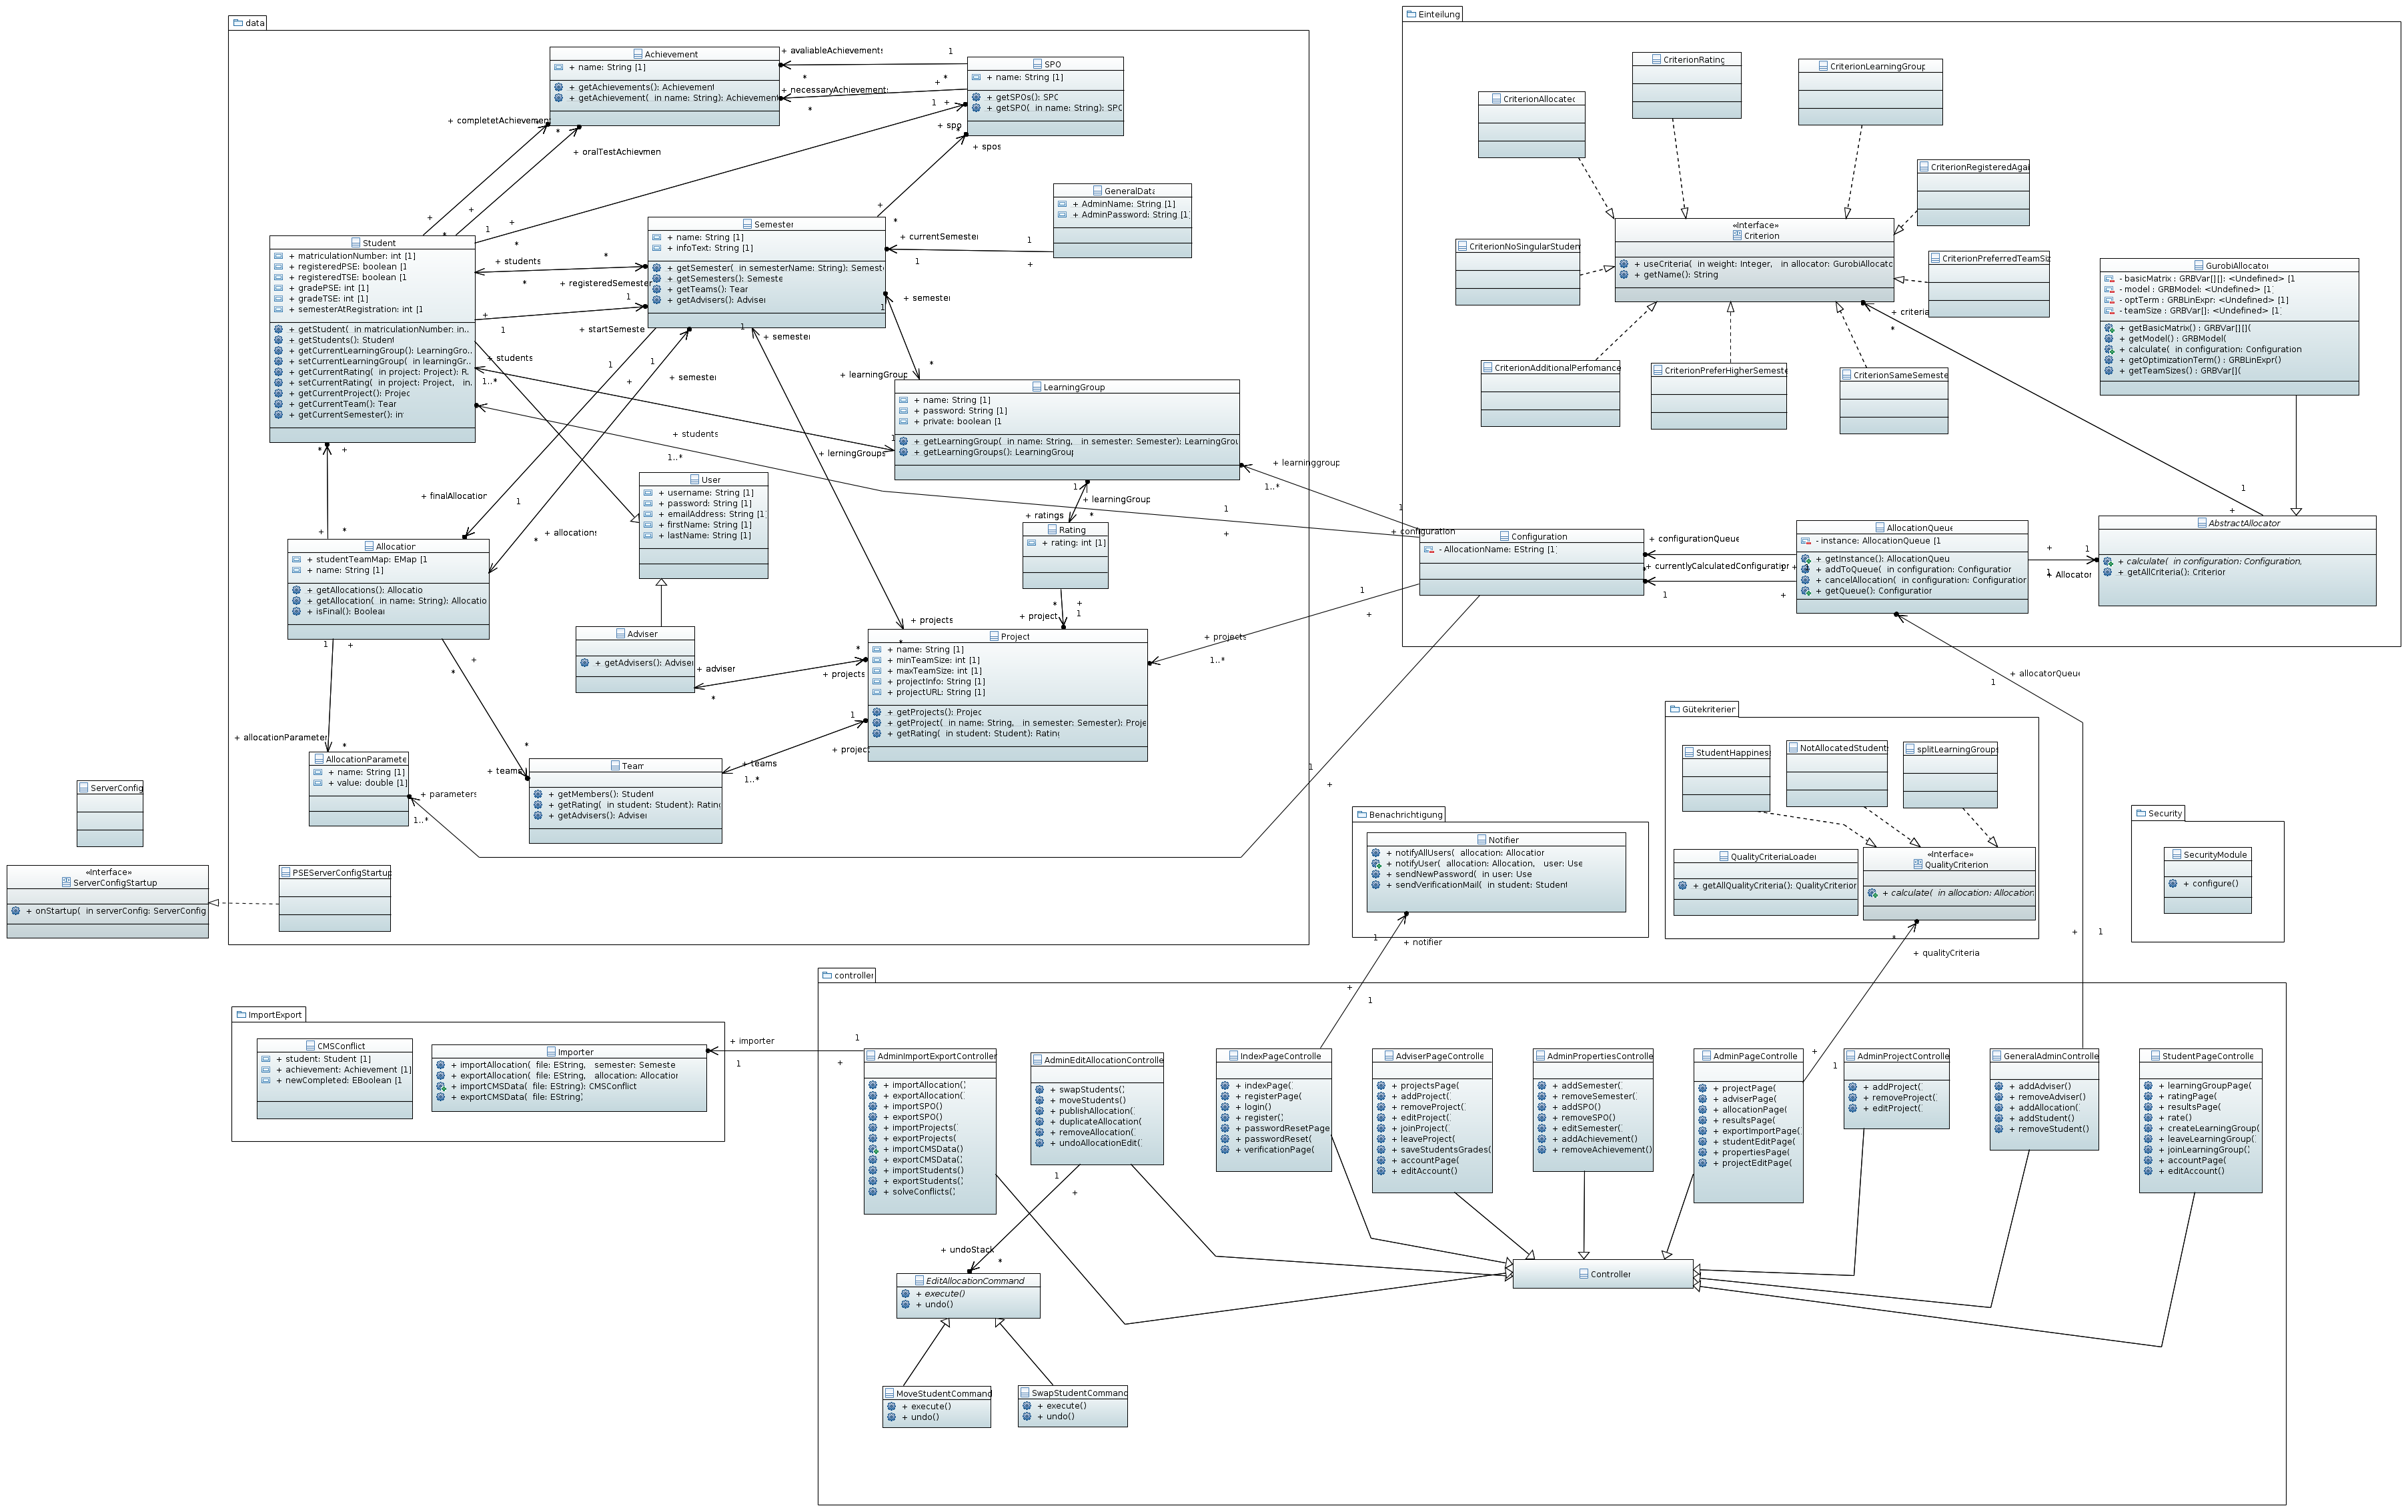
\includegraphics[width=\linewidth]{bilder/Class_Diagram.PNG}
\caption{Vollständiges Klassendiagramm}
\label{uml:classDiagram}
\end{sidewaysfigure}

\begin{sidewaysfigure}[!htb]
\centering
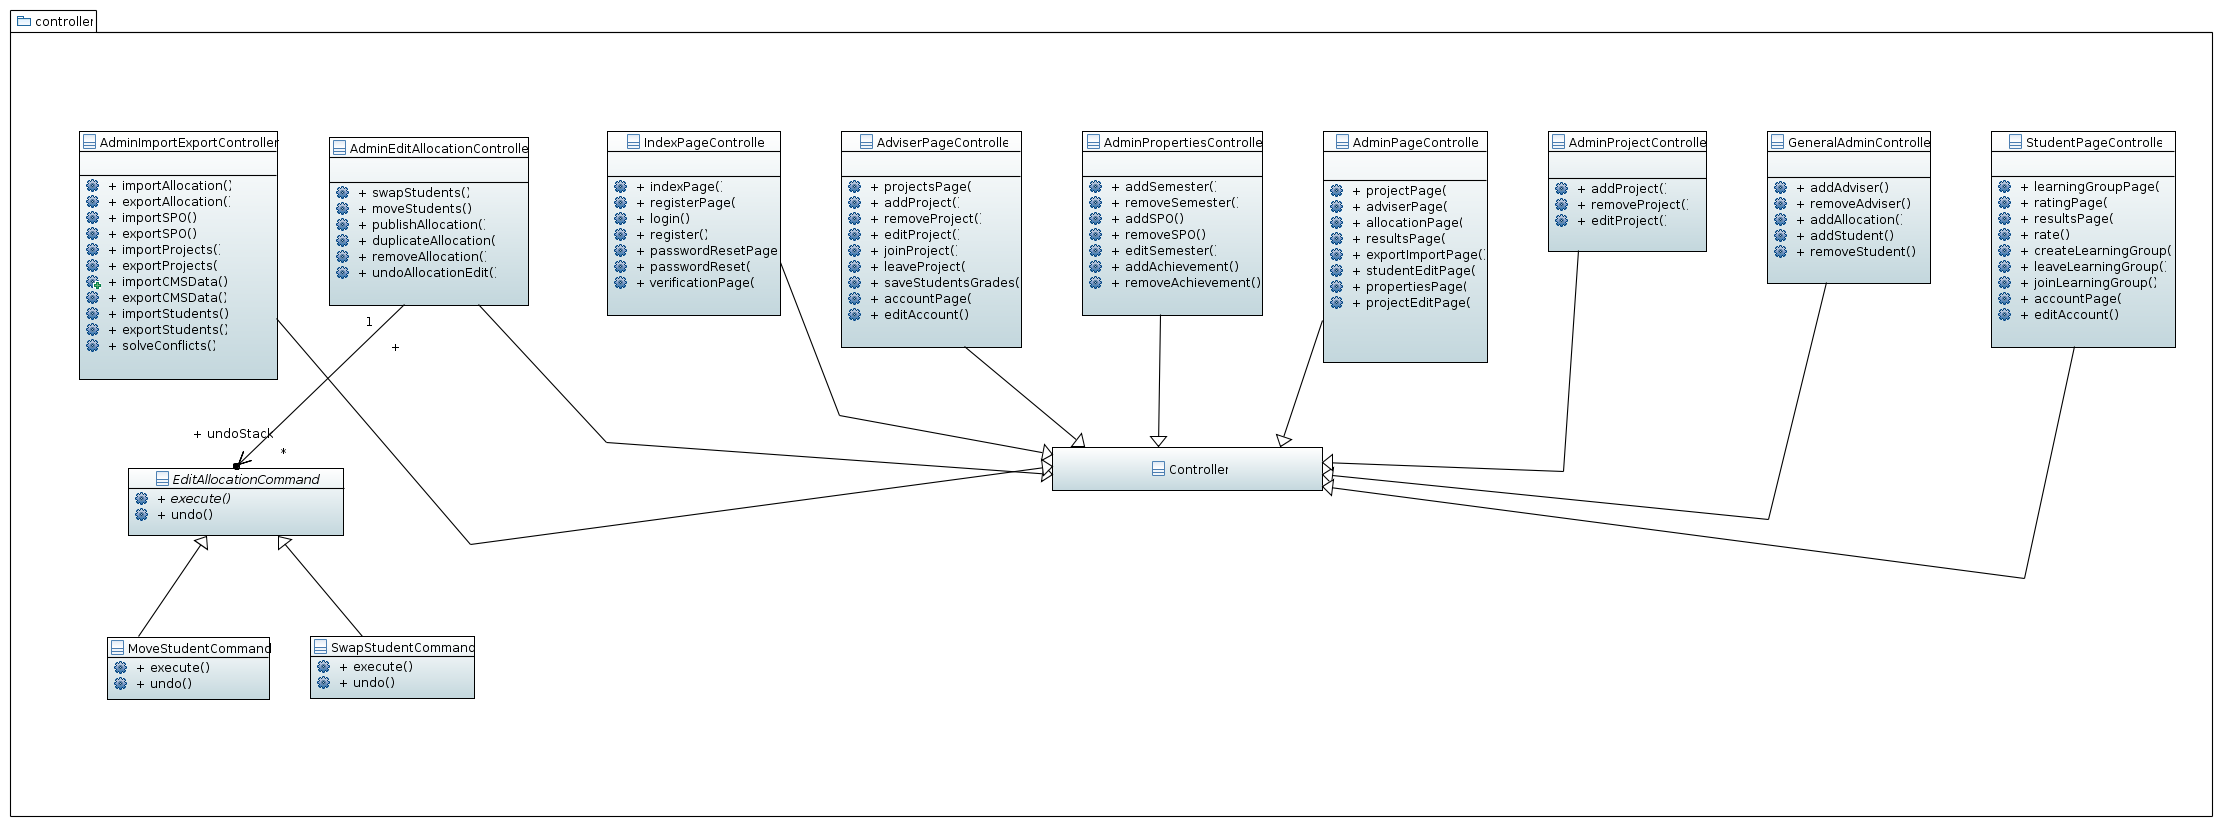
\includegraphics[width=\linewidth]{bilder/controller.png}
\caption{Controller}
\label{uml:controller}
\end{sidewaysfigure}

\begin{figure}[!htb]
\centering
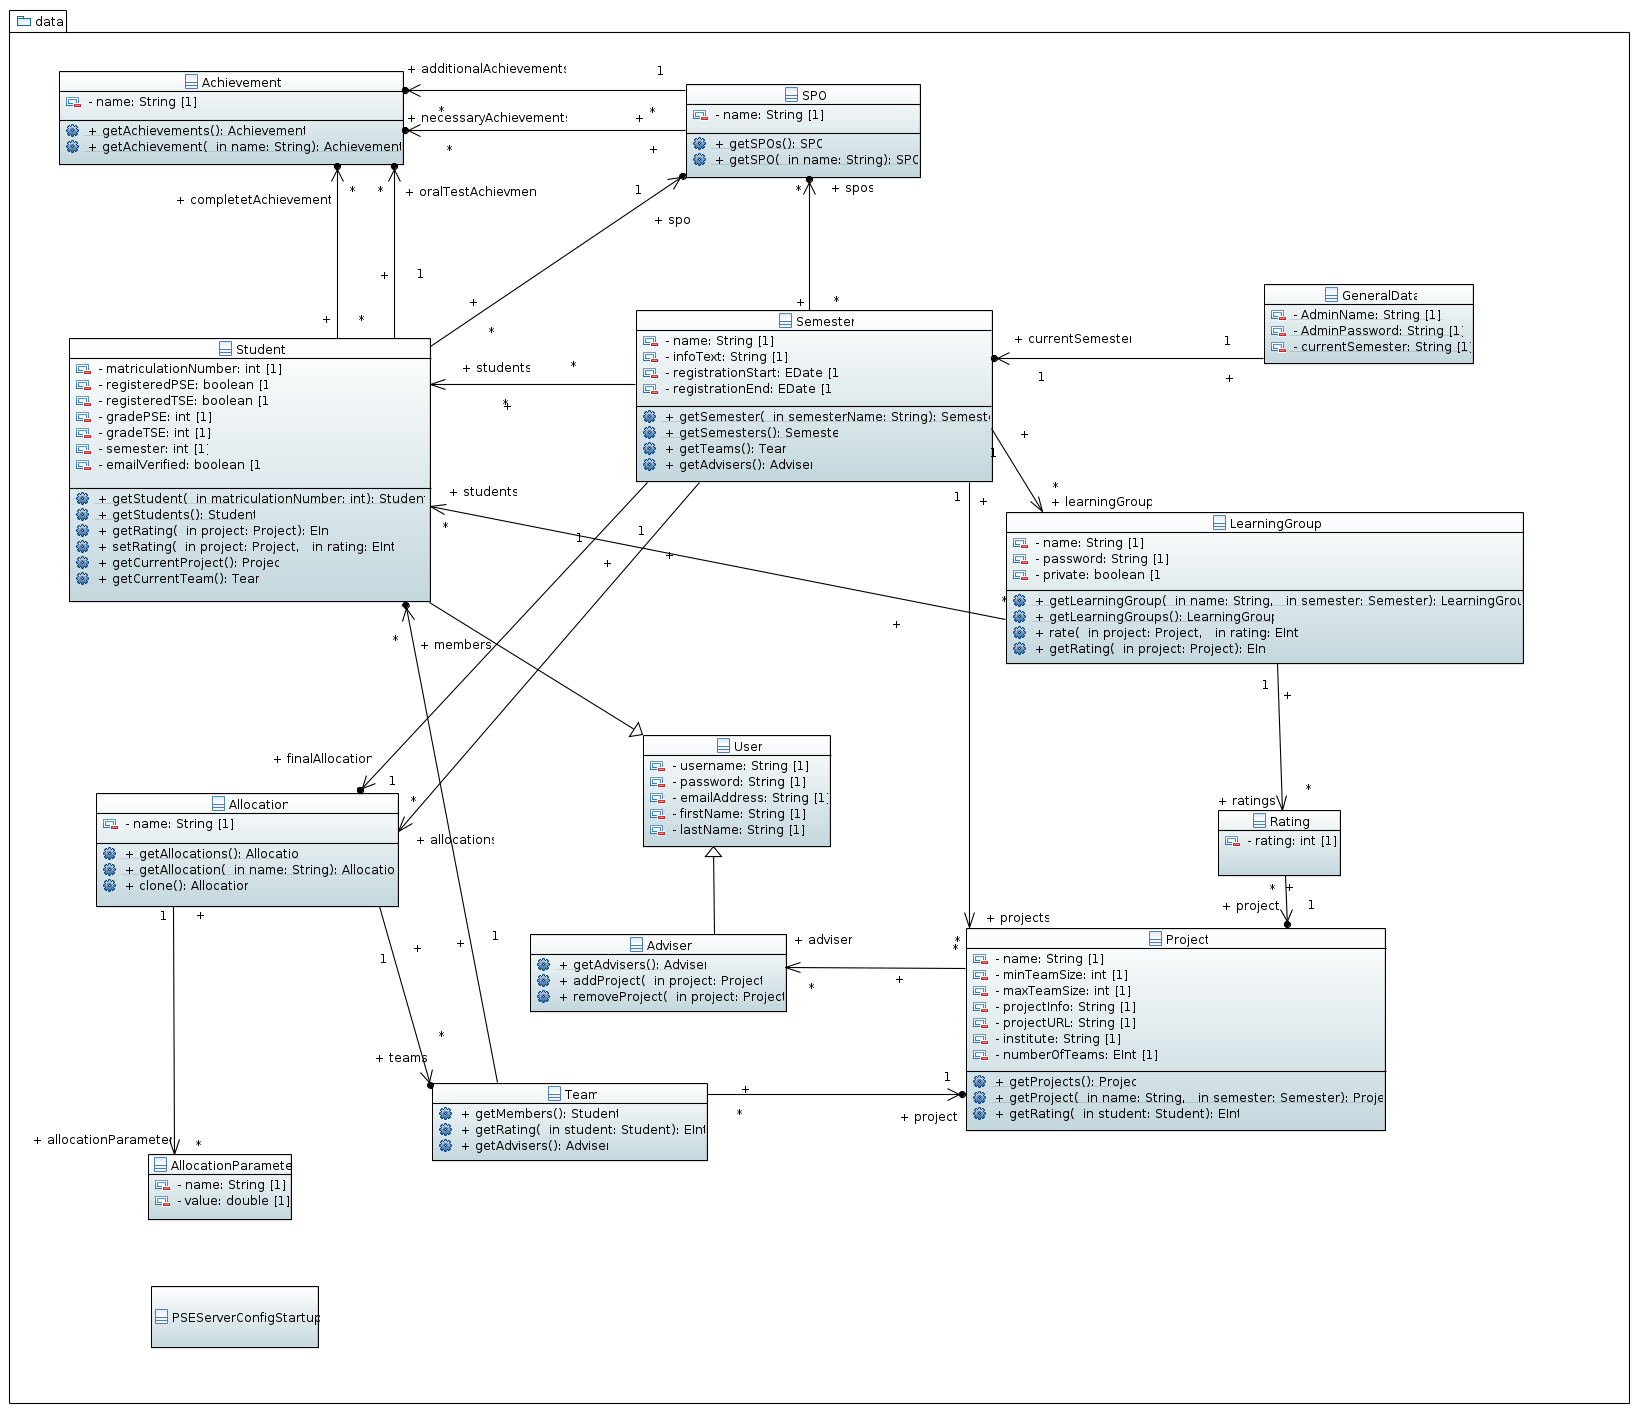
\includegraphics[width=\linewidth]{bilder/daten.png}
\caption{Datenmodell}
\label{uml:data}
\end{figure}

\begin{sidewaysfigure}[!htb]
\centering
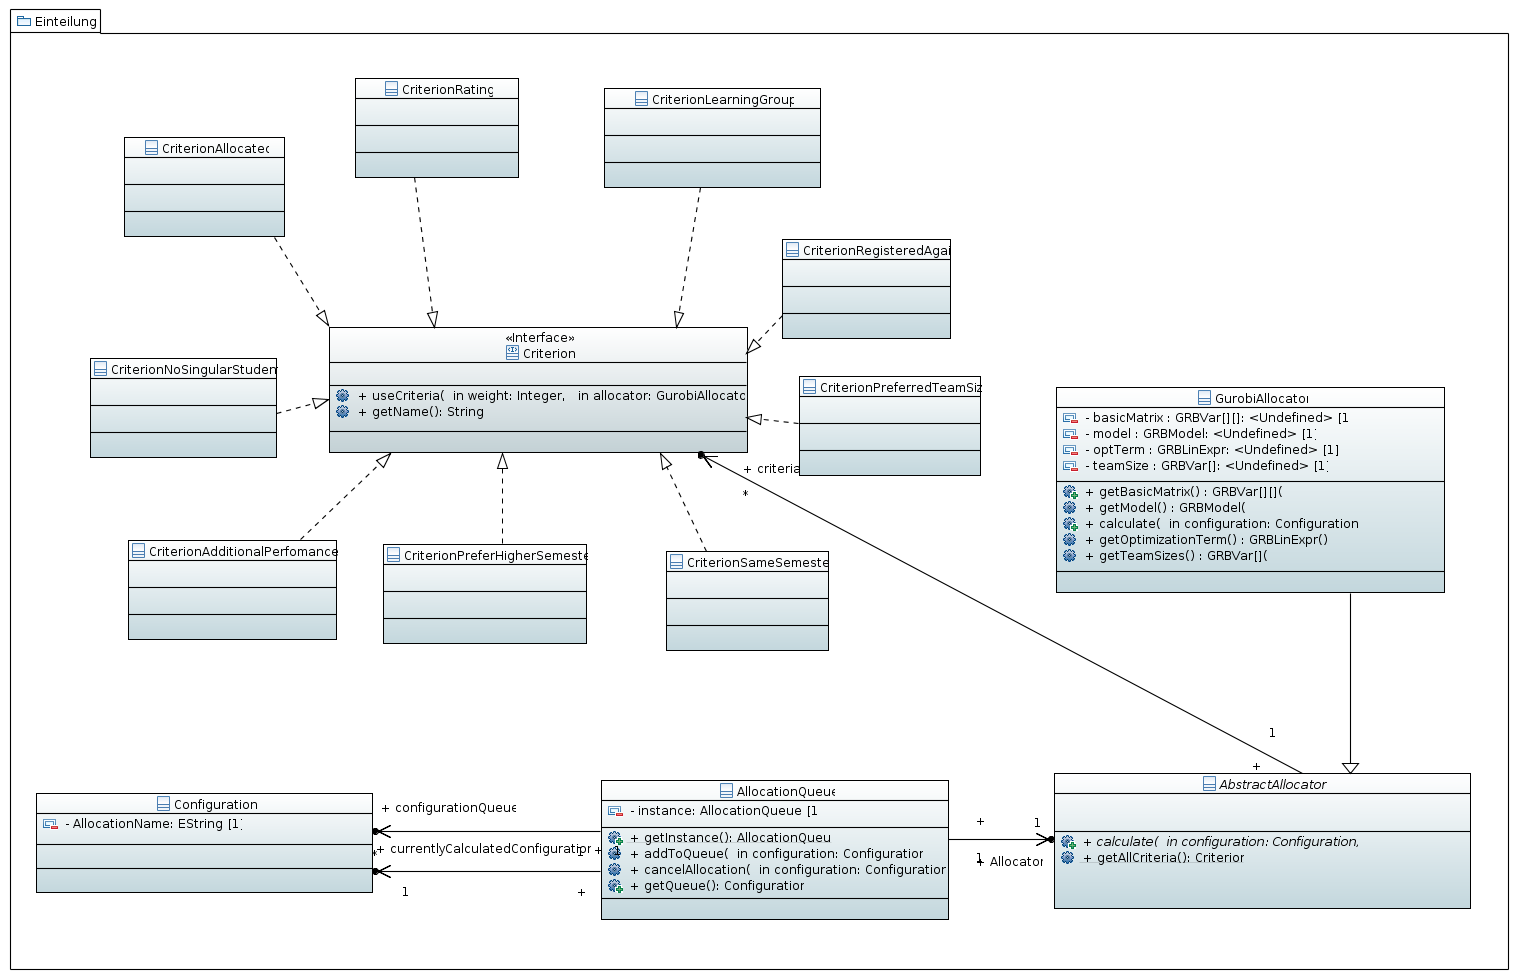
\includegraphics[width=\linewidth]{bilder/einteilung.png}
\caption{Einteilung}
\label{uml:allocation}
\end{sidewaysfigure}

\begin{figure}[!htb]
\centering
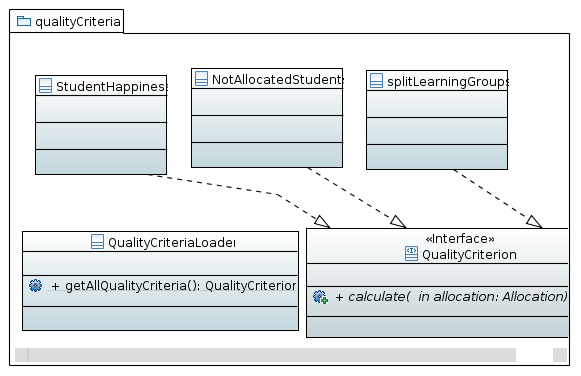
\includegraphics[width=\linewidth]{bilder/qualityCriteria.png}
\caption{Qualitätskriterien}
\label{uml:qualityCriteria}
\end{figure}

\begin{figure}[!htb]
\centering
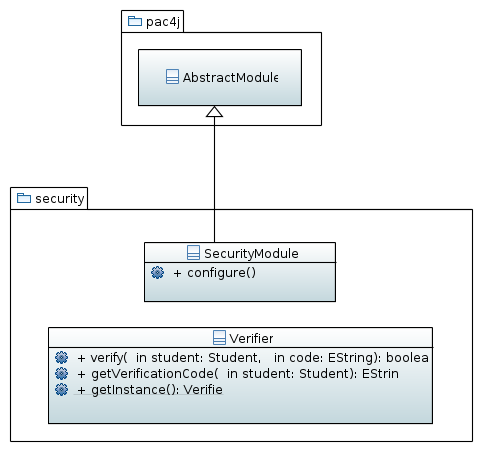
\includegraphics[width=\linewidth]{bilder/security.png}
\caption{Sicherheit}
\label{uml:Sicherheit}
\end{figure}

\begin{figure}[!htb]
\centering
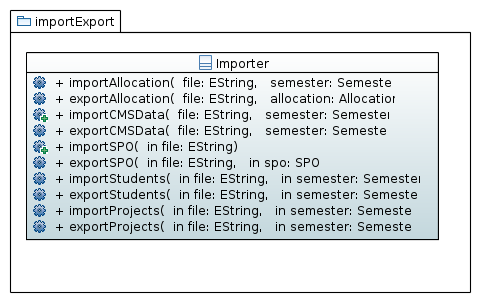
\includegraphics[width=\linewidth]{bilder/importExport.png}
\caption{Im- und Export}
\label{uml:imExport}
\end{figure}




\begin{sidewaysfigure}[!htb]
\centering
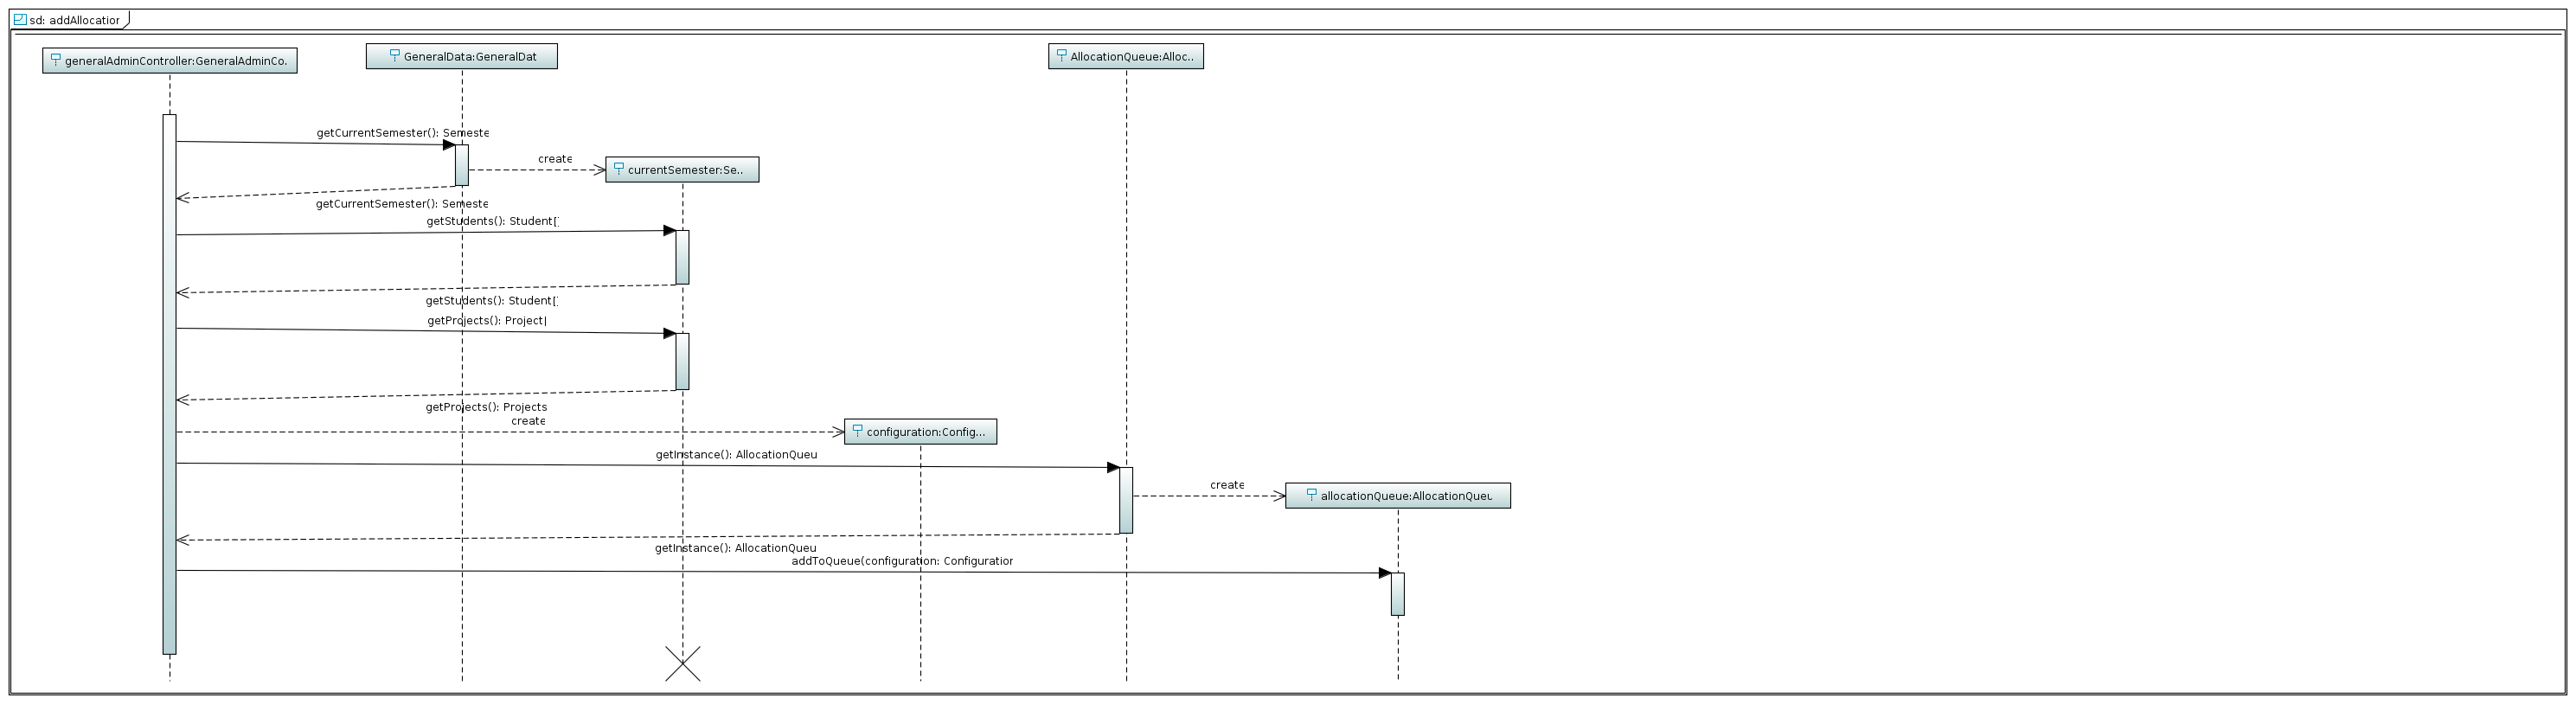
\includegraphics[width=\linewidth]{bilder/seqAddAllocation.png}
\caption{Add Allocation}
\label{seq:addAlloction}
\end{sidewaysfigure}

\begin{sidewaysfigure}[!htb]
\centering
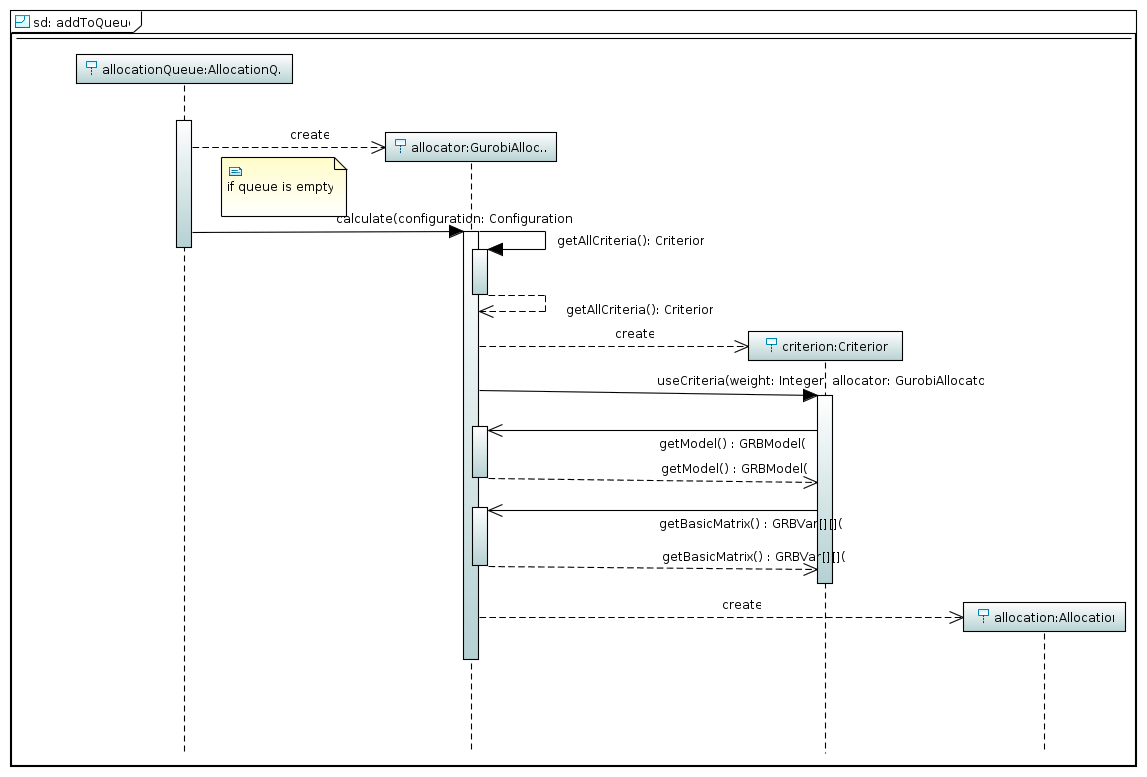
\includegraphics[width=\linewidth]{bilder/seqaddToQueue.png}
\caption{Add to Queue}
\label{seq:addToQueue}
\end{sidewaysfigure}
\end{document}\grid
\grid
